%!TeX encoding = UTF-8 Unicode
\documentclass{article}
\usepackage[pdftex]{graphicx} %for embedding images
\usepackage{url} %for proper url entries
\usepackage[bookmarks, colorlinks=false, pdfborder={0 0 0}, pdftitle={Laboratory ML Project 02}, pdfauthor={Nhut-Nam Le}, pdfsubject={Introduction to Machine Learning}, pdfkeywords={report, exercises}]{hyperref} %for creating links in the pdf version and other additional pdf attributes, no effect on the printed document
%\usepackage[final]{pdfpages} %for embedding another pdf, remove if not required
\usepackage[utf8]{inputenc}
\usepackage[english, vietnamese]{babel}
\usepackage{float}
\usepackage{fancyhdr}
\usepackage{pythonhighlight}
\usepackage[left=3cm, right=3cm, top=1.5cm, bottom=1.5cm]{geometry}
\usepackage{parskip}
\usepackage{tikz}
\usepackage{hyperref}
\usepackage[]{algorithm2e}
\usepackage[noend]{algpseudocode}
\usepackage{amsmath}
\usepackage{amsfonts}

\usepackage{listings}
\usepackage{color}

\definecolor{dkgreen}{rgb}{0,0.6,0}
\definecolor{gray}{rgb}{0.5,0.5,0.5}
\definecolor{mauve}{rgb}{0.58,0,0.82}

\newcommand\T{\rule{0pt}{2.6ex}}       % Top strut
\newcommand\B{\rule[-1.2ex]{0pt}{0pt}} % Bottom strut


\lstset{frame=tb,
	language=Java,
	aboveskip=3mm,
	belowskip=3mm,
	showstringspaces=false,
	columns=flexible,
	basicstyle={\small\ttfamily},
	numbers=none,
	numberstyle=\tiny\color{gray},
	keywordstyle=\color{blue},
	commentstyle=\color{dkgreen},
	stringstyle=\color{mauve},
	breaklines=true,
	breakatwhitespace=true,
	tabsize=3
}

\setlength{\parindent}{15pt}
\setlength{\headheight}{15.2pt}
\pagestyle{fancy}
\lhead[<even output>]{NHẬP MÔN HỌC MÁY}
\rhead[<even output>]{BÁO CÁO ĐỒ ÁN THỰC HÀNH 02}
\title{research-outline}
\author{Nhut-Nam Le}
\date{2021}
\begin{document}
	\begin{titlepage}
		\begin{center}
			% Top of the page
			\large{\textbf{ĐẠI HỌC KHOA HỌC TỰ NHIÊN, ĐHQG-HCM\\KHOA CÔNG NGHỆ THÔNG TIN\\BỘ MÔN KHOA HỌC MÁY TÍNH}}\\
			
\includegraphics[width=0.75\textwidth]{images/khtn.png}\\
			% Title
			\large \textbf{NHẬP MÔN HỌC MÁY}\\[0.1in]
			\huge \textbf{BÁO CÁO ĐỒ ÁN THỰC HÀNH}\\[0.1in]
			\huge \textbf{CLASSIFICATION - PHÂN LỚP}\\[0.1in]
			\vfill
			\normalsize
			% Submitted by
			\normalsize
			% Lecturers
			\textbf{Giảng viên lý thuyết}\\
			{\textbf{TS.} Bùi Tiến Lên}\\[0.1in]
			% Teacher Assistant
			\textbf{Giảng viên hướng dẫn}\\
			\vspace{0.1in}
			{Dương Nguyễn Thái Bảo, Nguyễn Ngọc Đức, Nguyễn Tiến Huy, Lê Thanh Phong}\\[0.1in]
			\textbf{Sinh viên thực hiện} \\
			\vspace{0.1in}
			% Submitted by
			{Vương Gia Bảo, Ngô Xuân Kiên, Lê Nhựt Nam, Nguyễn Viết Dũng}\\[0.1in]
			% Date time when written report
			\vfill
			Tháng 5 năm 2021
		\end{center}
	\end{titlepage}
	\newpage
	% End Title4
	
	\pagenumbering{roman} %numbering before main content starts
	\cleardoublepage
	%\pagebreak
	\phantomsection
	\addcontentsline{toc}{section}{Lời cảm ơn}
	\section*{Lời cảm ơn}
	\vspace{1.0in}
	\begingroup
	\setlength{\parindent}{0pt}
	\qquad Trong quá trình thực hiện đồ án này, chúng em đã nhận được rất nhiều sự giúp đỡ cũng như hỗ trợ từ các thầy cô Trường Đại học Khoa học Tự nhiên, ĐHQG-HCM và các bạn bè trong lớp Nhập môn Học Máy. Chúng em xin bày tỏ lòng cảm ơn chân thành đến mọi người vì đã giúp đỡ hướng dẫn, chỉ bảo rất tận tình.
	
	\qquad Đặc biệt, chúng em xin bày tỏ lòng biết ơn sâu sắc đến các thầy cô khoa Công nghệ Thông tin, cụ thể hơn là thầy Bùi Tiến Lên và các thầy hướng dẫn đã giảng dạy rất nhiệt, cung cấp nhiều slides, tài nguyên học tập cần thiết, tạo điều kiện tốt nhất để chúng em có thể hoàn thành được đồ án này.
	
	\qquad Trong quá trình, viết báo cáo này, chúng em không thể tránh khỏi nhiều thiếu sót, hy vọng mong nhận được góp ý từ thầy để chúng em tiếp tục hoàn thiện hơn đối với đồ án này, cũng như rút kinh nghiệm cho những đồ án, những báo cáo kế tiếp.
	
	\vspace{1.0in}
	\textbf{Đại học Khoa học Tự nhiên, ĐHQG-HCM.}\\
	Vương Gia Bảo, Ngô Xuân Kiên, Lê Nhựt Nam, Nguyễn Viết Dũng\\
	Tháng 4 năm 2021\\
	\endgroup
	
	\newpage
	\tableofcontents
	\newpage
	\pagenumbering{arabic} %reset numbering to normal for the main content
	\setcounter{secnumdepth}{0}
	
	\section{Thông tin nhóm}
	\begin{table}[H]
		\centering
		\begin{tabular}{ | p{1cm} |  p{3cm} | p{5cm} | p{5cm}  |}\hline
			STT	& MSSV & Họ tên đầy đủ & Email liên lạc \\\hline
			1 & 18120009 & Vương Gia Bảo & 18120009@student.hcmus.edu.vn  \\ \hline
			2 & 18120045 & Ngô Xuân Kiên & 18120045@student.hcmus.edu.vn \\ \hline
			3 & 18120061 & Lê Nhựt Nam & 18120061@student.hcmus.edu.vn  \\ \hline
			4 & 18120167 & Nguyễn Viết Dũng &  18120167@student.hcmus.edu.vn \\ \hline
		\end{tabular}
	\end{table}
	\section{Phân công công việc}
	\begin{table}[H]
		\begin{tabular}{ | l | l | l | p{5.5cm} | p{3cm} |}
			\hline
			STT & MSSV & Họ tên & Nội dung công việc & Mức độ hoàn thành  \\ \hline
			1 & 18120009 & Vương Gia Bảo & Thu thập dữ liệu, đọc hiểu source, báo cáo Introduction Paper &  100\%\T\B\\ \hline
			2 & 18120045 & Ngô Xuân Kiên & Thu thập dữ liệu, đọc hiểu source, báo cáo Related Work Paper & 100\%\T\B \\ \hline
			3 & 18120061 & Lê Nhựt Nam & Thu thập dữ liệu, đọc hiểu source, báo cáo & 100\%\T\B \\ \hline
			4 & 18120167 & Nguyễn Viết Dũng &  Thu thập dữ liệu, đọc hiểu source, báo cáo experimental setup & 100\%\T\B \\ \hline
		\end{tabular}
	\end{table}
	\section{Tiêu chí đánh giá đồ án}
	\subsection{Bảng tiêu chí cho đồ án}
	\begin{table}[H]
		\begin{tabular}{ | p{5cm} | p{6.25cm} | p{3cm} |}\hline
			Tên tiêu chí đồ án & Nội dung tiêu chí & Mức độ hoàn thiện  \T\B\\\hline
			Nhận diện bài toán & Sinh viên cần tìm hiểu bài toán và dữ liệu được giao
			nhằm xác định nội dung và ý nghĩa bài toán thực tế cần giải quyết. Thông
			qua đó, sinh viên có khả năng ánh xạ vấn đề thực tế sang bài toán lập trình & 100\%  \T\B\\\hline
			Giải quyết vấn đề & Sinh viên được yêu cầu đưa ra các giải pháp và hướng
			tiếp cận nhằm giải quyết được yêu cầu bài toán thực tế & 100\%  \T\B\\\hline
			Xử lý và phân tích dữ liệu & Sinh viên có khả năng xử lý các công cụ phân
			tích dữ liệu tự động nhằm tìm ra các thông tin hữu ích, các đặc trưng tiềm ẩn
			ảnh hưởng để mục tiêu bài toán &100\%  \T\B\\\hline
			Thiết kế và cài đặt các thuật toán máy học & Sinh viên được yêu cầu có
			khả năng đề xuất, triển khai và giải thích các thuật toán máy học nhằm giải
			quyết bài toán được giao & 100\%  \T\B\\\hline
		\end{tabular}
	\end{table}
	\subsection{Bảng yêu cầu cho đồ án}
	\begin{table}[H]
		\begin{tabular}{ | p{5cm} | p{6.5cm} | p{3cm} |}\hline	
			Tên yêu cầu & Nội dung yêu cầu & Mức độ hoàn thiện  \T\B\\\hline
			Phân tích dữ liệu & Phân tích kỹ bài toán và tập dữ liệu hình ảnh được cung cấp. Chọn lựa và
			trình bày kiểu mạng nơron để giải quyết bài toán. & 100\%  \T\B\\\hline
			Cài đặt thuật toán & Cài đặt mạng Nơron. & 100\%  \T\B\\\hline
			Trình bày kết quả và nhận xét & Báo cáo kết quả đạt đưoc sau quá trình phân tích và cài đặt. & 100\%  \T\B\\\hline
		\end{tabular}
	\end{table}	
	\section{Nội dung báo cáo}
	\section{1. Tổng quan về bài toán}
	\qquad Trong nộng nghiệp, năng suất của cây trồng phụ thuộc rất nhiều vào thời
	tiết, chế độ chăm sóc, sâu bệnh,... để tăng năng suất người trồng cần có những
	biện pháp hạn chế những tác động của các yếu tố trên.
	
	Tuy nhiên, bản thân cây trồng cũng có những loại bệnh nhất định và thường
	biểu hiện ra bên ngoài trên thân, lá... những biểu hiện đó bất thường trên cây
	trồng thường liện quan tới một loại bệnh nào đó.
	
	Nhằm giúp người trồng xác định được loại bệnh đang có trên cây trồng,
	sinh viên được cung cấp tập dữ liệu hình ảnh về các loại bệnh trên cây và tập dữ
	liệu đã được xác định được loại bệnh (train.csv và test.csv) bao gồm 4 loại:
	\begin{itemize}
		\item Healthy
		\item Combinations
		\item Rust
		\item Scab
	\end{itemize}
	Dữ liệu có 3 tập tin
	\begin{itemize}
		\item train.csv
		\begin{itemize}
			\item image\_id: the foreign key
			\item combinations: one of the target labels
			\item healthy: one of the target labels
			\item rust: one of the target labels
			\item scab: one of the target labels
		\end{itemize}
		\item test.csv
		\begin{itemize}
			\item image\_id: the foreign key
		\end{itemize}
		\item sample\_submission.csv
		\begin{itemize}
			\item image\_id: the foreign key
			\item combinations: one of the target labels
			\item healthy: one of the target labels
			\item rust: one of the target labels
			\item scab: one of the target labels
		\end{itemize}
	\end{itemize}
	Thư mục images chứa tất cả ảnh huấn luyện (train images) và ảnh kiểm tra (test images), với định dạng là .jpg
	\section{2. Công cụ và môi trường thực thi}
	\qquad Với yêu cầu thực hiện của đồ án, để thuận tiện cho làm việc, trao đổi, nhóm chọn môi trường Google Colab hỗ trợ để chạy Jupyter Notebook, mặc khác là để đảm bảo rằng đầy đủ các thư viện cần thiết cho đồ án.
	
	Đối với tác vụ tính toán số học, xử lý bảng dữ liệu, nhóm chọn hai thư viện mạnh mẽ, Numpy và Pandas hỗ trợ trong việc đọc các đường dẫn, tính toán kernel, ...
	
	Đối với tác vụ khai thông tin, phân tích dữ liệu bằng các công cụ trực quan hóa dữ liệu, nhóm sử dụng thư viện Matplotlib, Seaborn và Plotly trong việc vẽ các biểu đồ (chart), sơ đồ (diagram), histogram,...
	
	Đối với tác vụ đọc, ghi, xử lý dữ liệu hình ảnh, nhóm chọn thư viện Python-OpenCV, scikit-image để triển khai các phép biến đổi tăng cường hình ảnh như phát hiện biên cạnh bằng giải thuật Canny (The Canny Edge Detector), Đóng bouding boxes, Lật ảnh (Flipping image), Làm trơn hình ảnh (Bluring), Phép tính chập với kernel tùy chọn (Convolutional), ...
	
	Đối với tác vụ cài đặt Neural Networks, nhóm chọn thư viện Pytorch sử dụng GPU Google Colab trong việc cài đặt mô hình mạng, huấn luyện mô hình
	
	Đối với tác vụ đánh giá mô hình, nhóm sử dụng Sklearn hỗ trợ sử dụng một số độ đo trong việc đánh giá mô hình.
	
	\section{3. Khám phá cấu trúc dữ liệu}
	\qquad Để tự động trong việc xử lý dữ liệu, nhóm chọn cách download trực tiếp và lưu trữ vào bộ nhớ máy ảo Google Colab, sử dụng package gdown để download dữ liệu chuẩn bị sẵn ở Google Drive (Link Google Drive này khác với Link được cung cấp, vì để đảm bảo rằng đường dẫn sẽ được hoạt động tốt trong thời gian lâu dài)
	\begin{figure}[H]
		\centering
		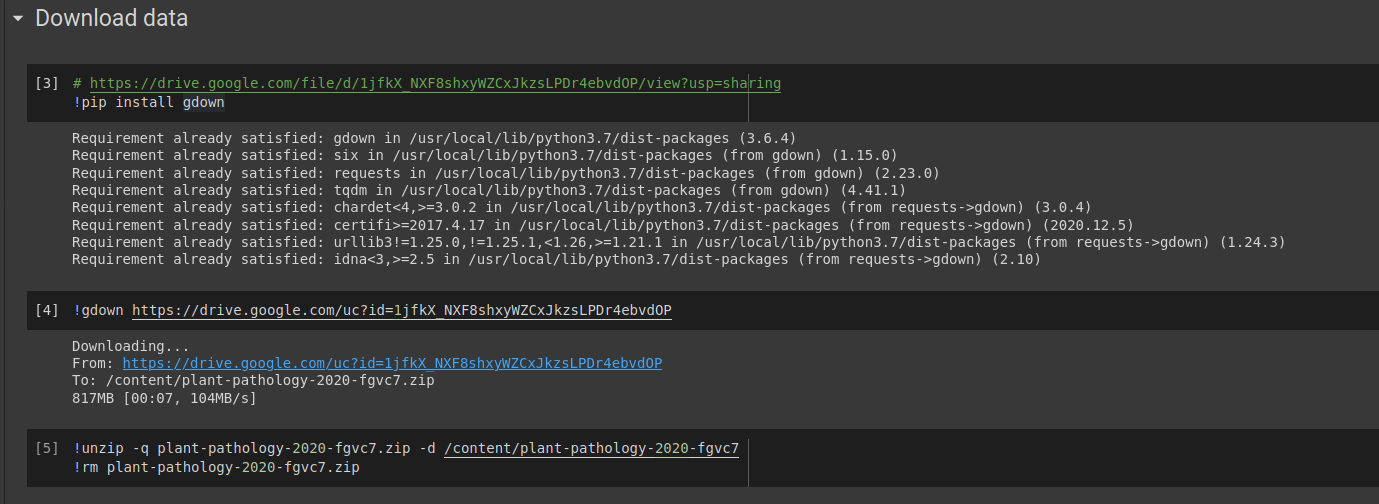
\includegraphics[width=0.75\linewidth]{images/download_plant_pathology_dataset.png}
		\label{fig:writing-thesis}
	\end{figure}
	Cài đặt các biến toàn cục lưu những thông tin về dữ liệu
	\begin{itemize}
		\item IMAGES\_PATH: đường dẫn đến thư mục images trong bộ dữ liệu, nơi chứa tất cả hình ảnh cho việc huấn luyện và kiểm tra mô hình
		\item SAMPLE\_SUBMISSION: đường dẫn đến file sample\_submission.csv
		\item TRAIN\_DATA: đường dẫn đến file train.csv
		\item TEST\_DATA: đường dẫn đến file test.csv
	\end{itemize}
	Dùng Pandas đọc dữ liệu từ hai tập tin .csv, nhóm cũng dùng apply built-in method để tạo thêm một thuộc tính image\_path, chứa đường dẫn đến tập tin hình để tiện cho việc đọc dữ liệu
	\begin{figure}[H]
		\centering
		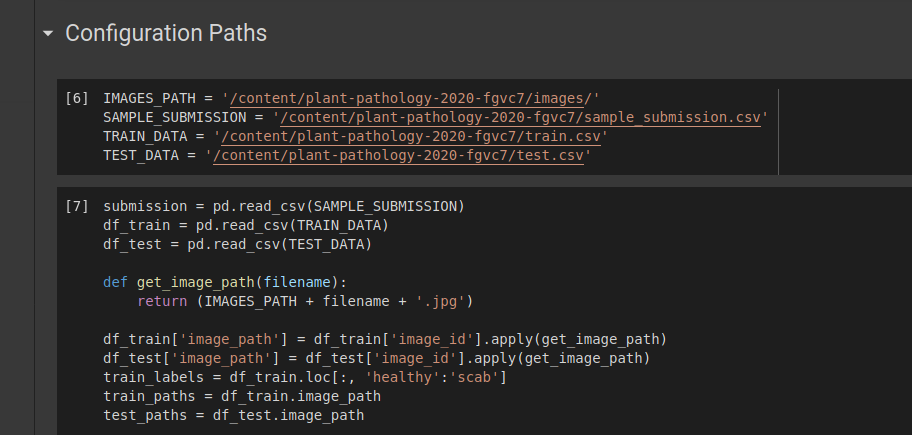
\includegraphics[width=0.75\linewidth]{images/configuration_paths.png}
		\label{fig:writing-thesis}
	\end{figure}
	Ta quan sát một số kết quả được thực hiện và thao tác dữ liệu phía trên
	\begin{figure}[H]
		\centering
		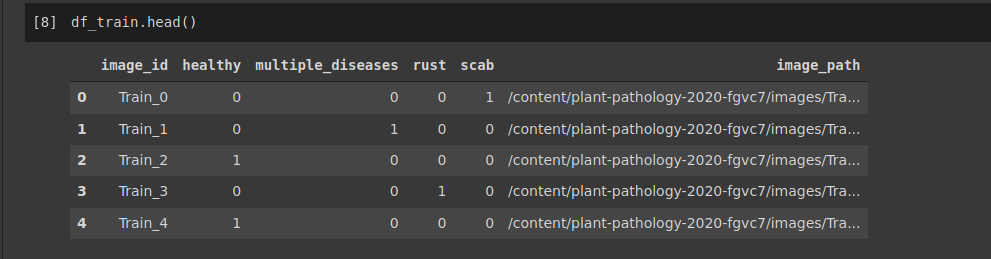
\includegraphics[width=0.75\linewidth]{images/head_df_train.png}
		\label{fig:writing-thesis}
	\end{figure}
	\begin{figure}[H]
		\centering
		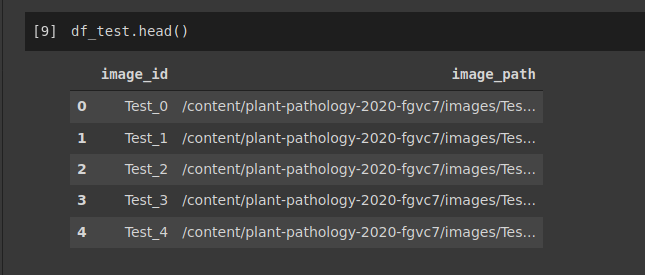
\includegraphics[width=0.75\linewidth]{images/head_df_test.png}
		\label{fig:writing-thesis}
	\end{figure}
	
	\section{4. Trực quan và phân tích dữ liệu}
	\subsection{4.1 Tổng quan về hình ảnh các loại bệnh}
	\textbf{Chọn ngẫu nhiên những chiếc lá không bị bệnh - Healthy Leaf}
	
	Ta nhận thấy, những chiếc lá khỏe mạnh thường xanh tốt, bề mặt lá không có đặc điểm ngoại lai hay những điểm đốm vàng, những vết nứt, vảy...
	\begin{figure}[H]
		\centering
		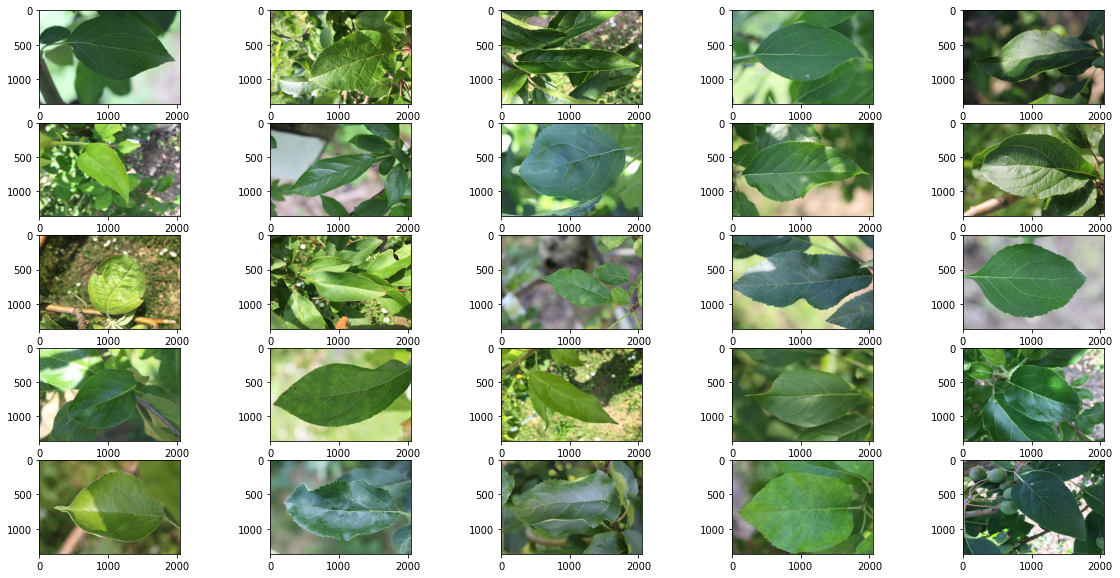
\includegraphics[width=1\linewidth]{images/sample_healthy_leaf.png}
		\caption{Một số mẫu hình ảnh về Healthy Leaf}
		\label{fig:writing-thesis}
	\end{figure}
	\begin{python}
		def plot_patches(data, size_selection, width_size, height_size, figure_size, type_patches=0, is_positive=True):
		fig, ax = plt.subplots(height_size, width_size, figsize=figure_size)
			if type_patches == 0:
				if is_positive:
					healthy_selection = np.random.choice(
					data[data.healthy == 1].index.values, size=size_selection, replace=False)
					for i in range(height_size):
						for j in range(width_size):
						idx = healthy_selection[j + width_size*i]
						image = io.imread(data.loc[idx, 'image_path'])
						ax[i, j].imshow(image)
					ax[i, j].grid(False)
				else:
					non_healthy_selection = np.random.choice(
					data[data.healthy == 0].index.values, size=size_selection, replace=False)
					for i in range(height_size):
						for j in range(width_size):
							idx = non_healthy_selection[j + width_size*i]
							image = io.imread(data.loc[idx, 'image_path'])
							ax[i, j].imshow(image)
							ax[i, j].grid(False)
	\end{python}
	\textbf{Chọn ngẫu nhiên những chiếc lá bị bệnh tổ hợp - Multiple Diseases Leaf}
	
	Ta có thể thấy những chiếc lá mắc tổ hợp nhiều bệnh thường có đặc điểm của một hoặc nhiều bệnh như bệnh gỉ sắt (rust), bệnh vảy (scab)
	\begin{figure}[H]
		\centering
		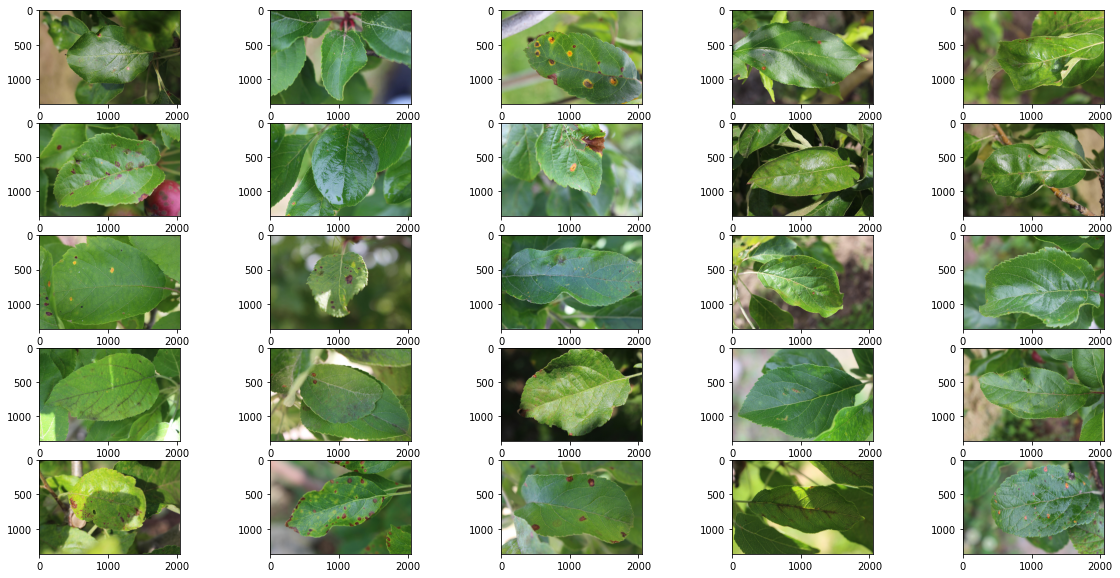
\includegraphics[width=1\linewidth]{images/sample_multiple_diseases_leaf.png}
		\caption{Một số mẫu hình ảnh về Multiple Diseases Leaf}
		\label{fig:writing-thesis}
	\end{figure}
	\begin{python}
		def plot_patches(data, size_selection, width_size, height_size, figure_size, type_patches=0, is_positive=True):
			if type_patches == 1:
				if is_positive:
				multiple_diseases_selection = np.random.choice(
				data[data.multiple_diseases == 1].index.values, size=size_selection, replace=False)
				for i in range(height_size):
					for j in range(width_size):
						idx = multiple_diseases_selection[j + width_size*i]
						image = io.imread(data.loc[idx, 'image_path'])
						ax[i, j].imshow(image)
						ax[i, j].grid(False)
				else:
					non_multiple_diseases_selection = np.random.choice(
					data[data.multiple_diseases == 0].index.values, size=size_selection, replace=False)
					for i in range(height_size):
						for j in range(width_size):
							idx = non_multiple_diseases_selection[j + width_size*i]
							image = io.imread(data.loc[idx, 'image_path'])
							ax[i, j].imshow(image)
							ax[i, j].grid(False)
	\end{python}
	\textbf{Chọn ngẫu nhiên những chiếc lá bị bệnh Rust - Rust Diseases Leaf}
	
	Ta nhận thấy, những chiếc lá bị bệnh "gỉ sắt" có một vài đốm màu vàng nâu trên khắp mặt lá. Bệnh gỉ sắt được định nghĩa là "một loại bệnh, đặc biệt là đối với ngũ cốc và các loại cỏ khác, đặc trưng bởi các bào tử có mụn mủ màu gỉ sắt trên phiến lá và bẹ lá bị bệnh và do bất kỳ loại nấm gỉ sắt nào gây ra". Các đốm vàng là dấu hiệu nhiễm trùng của một loại nấm đặc biệt gọi là "nấm gỉ sắt". Rỉ sét cũng có thể được điều trị bằng một số phương pháp hóa học và không hóa học khi đã được chẩn đoán.
	\begin{figure}[H]
		\centering
		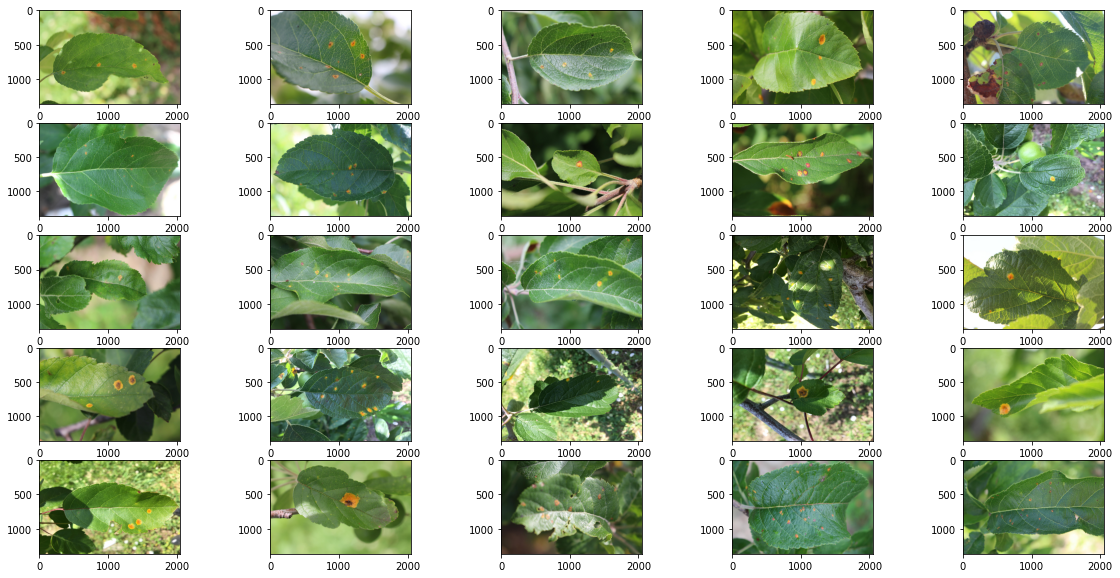
\includegraphics[width=1\linewidth]{images/sample_rust_leaf.png}
		\caption{Một số mẫu hình ảnh về Rust Diseases Leaf}
		\label{fig:writing-thesis}
	\end{figure}
	\begin{python}
		def plot_patches(data, size_selection, width_size, height_size, figure_size, type_patches=0, is_positive=True):
			if type_patches == 2:
				if is_positive:
					rust_selection = np.random.choice(
					data[data.rust == 1].index.values, size=size_selection, replace=False)
					for i in range(height_size):
						for j in range(width_size):
							idx = rust_selection[j + width_size*i]
							image = io.imread(data.loc[idx, 'image_path'])
							ax[i, j].imshow(image)
							ax[i, j].grid(False)
				else:
					non_rust_selection = np.random.choice(
					data[data.rust == 0].index.values, size=size_selection, replace=False)
					for i in range(height_size):
						for j in range(width_size):
							idx = non_rust_selection[j + width_size*i]
							image = io.imread(data.loc[idx, 'image_path'])
							ax[i, j].imshow(image)
							ax[i, j].grid(False)
	\end{python}
	\textbf{Chọn ngẫu nhiên những chiếc lá bị bệnh Scab - Scab Diseases Leaf}
	
	Ta nhận thấy, những chiếc lá bị “vảy” có những vết lớn màu nâu và những vết loang lổ khắp mặt lá. Bệnh vảy (scab) được định nghĩa là "bất kỳ bệnh thực vật nào khác nhau do nấm hoặc vi khuẩn gây ra và dẫn đến các đốm giống như vảy trên trái cây, lá hoặc rễ. Các đốm do bệnh như vậy gây ra". Các vết nâu trên lá là dấu hiệu của các bệnh nhiễm trùng do vi khuẩn/ nấm này. Sau khi được chẩn đoán, bệnh vảy có thể được điều trị bằng phương pháp hóa học (phun thuốc bảo vệ thực vật hóa học) hoặc không hóa chất (phun thuốc bảo vệ thực vật vi sinh).
	\begin{figure}[H]
		\centering
		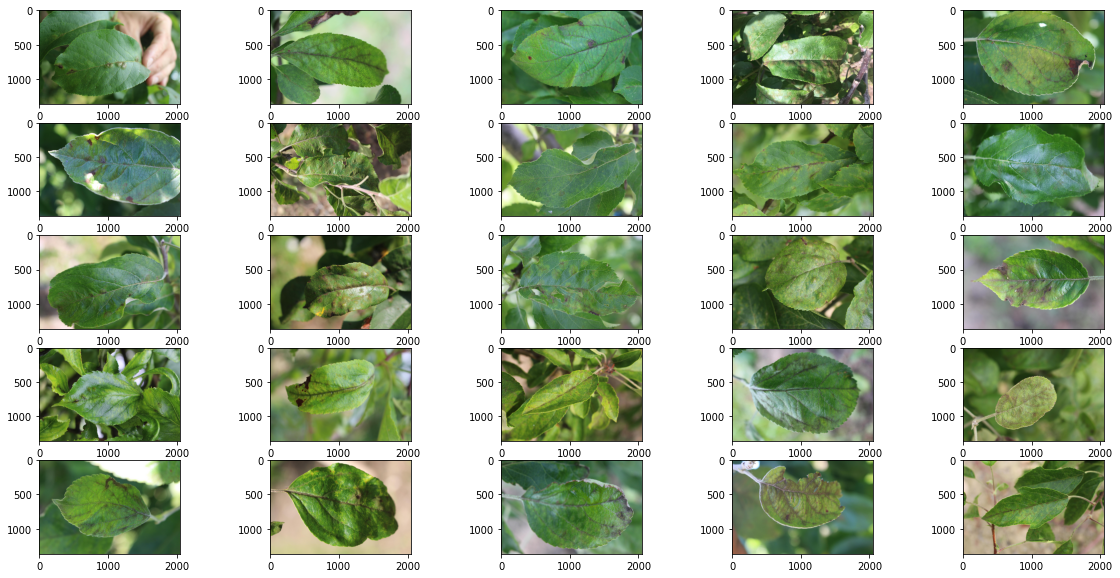
\includegraphics[width=1\linewidth]{images/sample_scab_diseases_leaf.png}
		\caption{Một số mẫu hình ảnh về Scab Diseases Leaf}
		\label{fig:writing-thesis}
	\end{figure}
	\begin{python}
		def plot_patches(data, size_selection, width_size, height_size, figure_size, type_patches=0, is_positive=True):
			if type_patches == 3:
				if is_positive:
					scab_diseases_selection = np.random.choice(
					data[data.scab == 1].index.values, size=size_selection, replace=False)
					for i in range(height_size):
						for j in range(width_size):
							idx = scab_diseases_selection[j + width_size*i]
							image = io.imread(data.loc[idx, 'image_path'])
							ax[i, j].imshow(image)
							ax[i, j].grid(False)
				else:
					non_scab_diseases_selection = np.random.choice(
					data[data.scab == 0].index.values, size=50, replace=False)
					for i in range(height_size):
						for j in range(width_size):
							idx = non_scab_diseases_selection[j + width_size*i]
							image = io.imread(data.loc[idx, 'image_path'])
							ax[i, j].imshow(image)
							ax[i, j].grid(False)
	\end{python}
	\subsection{4.2 Phân phối các kênh màu trên mẫu từ tập dữ liệu}
	Chọn ngẫu nhiên từ tập huấn luyện 500 hình ảnh lá cây để xét phân bố màu sắc gồm 3 kênh màu (RGB) của hình ảnh trong tập ảnh, với kích thước này là đủ lớn để suy ra tính chất của tập dữ liệu.
	\textbf{Phân bố kênh màu đỏ - Red Channel Distribution}
	\begin{figure}[H]
		\centering
		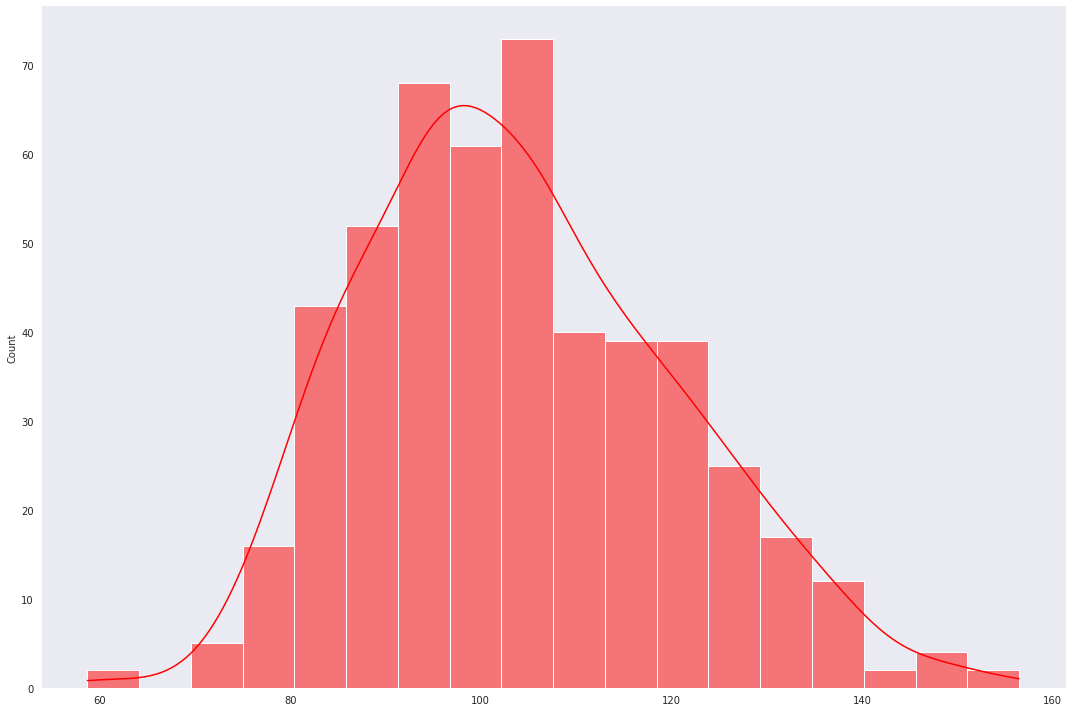
\includegraphics[width=1\linewidth]{images/red_channel_distribution.png}
		\caption{Phân phối kênh màu đỏ - Red Channel Distribution}
		\label{fig:writing-thesis}
	\end{figure}
	Nhận xét:
	\begin{itemize}
		\item Phân phối kênh màu đỏ có thể xấp xỉ bằng phân phối chuẩn
		\item Giá trị trung bình của kênh màu năm trong khoảng giá trị gần 100
		\item Giá trị nhỏ nhất khoảng 60, giá trị lớn nhất khoảng dưới 160
	\end{itemize}
	\textbf{Phân bố kênh màu xanh lá - Green Channel Distribution}
	\begin{figure}[H]
		\centering
		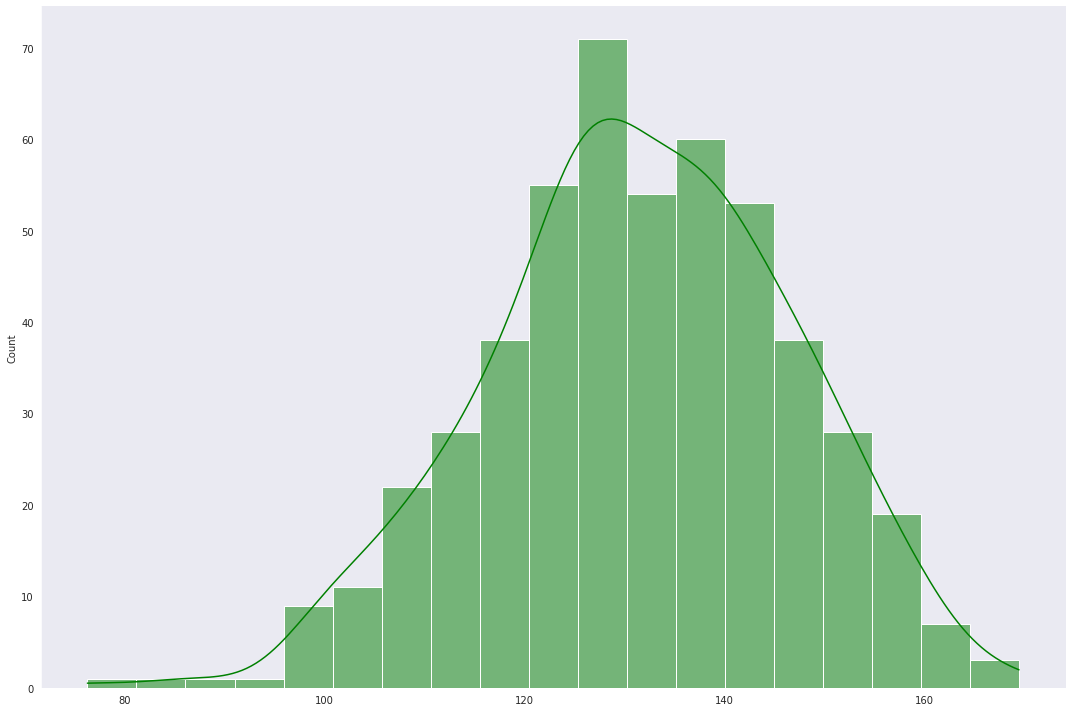
\includegraphics[width=1\linewidth]{images/green_channel_distribution.png}
		\caption{Phân phối kênh màu xanh lá - Green Channel Distribution}
		\label{fig:writing-thesis}
	\end{figure}
	Nhận xét:
	\begin{itemize}
		\item Phân phối kênh màu xanh lá có thể xấp xỉ bằng phân phối chuẩn
		\item Giá trị trung bình của kênh màu năm trong khoảng giá trị gần 130
		\item Giá trị nhỏ nhất khoảng 80, giá trị lớn nhất khoảng dưới 180
	\end{itemize}
	\textbf{Phân bố kênh màu xanh dương - Blue Channel Distribution}
	\begin{figure}[H]
		\centering
		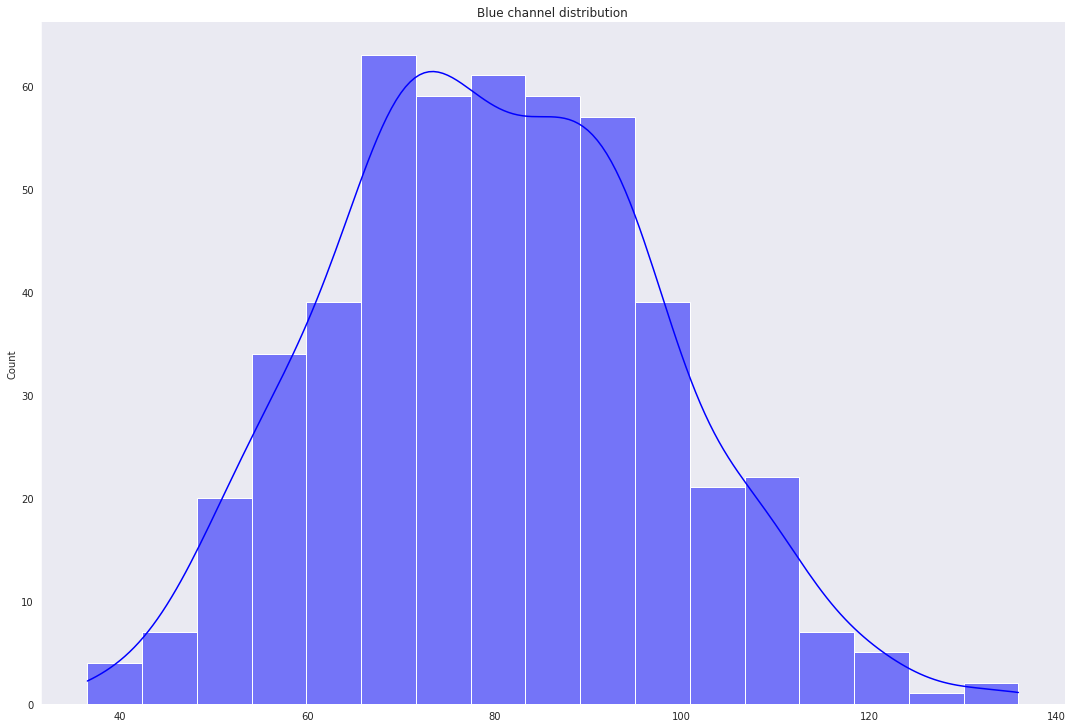
\includegraphics[width=1\linewidth]{images/blue_channel_distribution.png}
		\caption{Phân phối kênh màu xanh dương - Blue Channel Distribution}
		\label{fig:writing-thesis}
	\end{figure}
	Nhận xét:
	\begin{itemize}
		\item Phân phối kênh màu xanh dương có thể xấp xỉ bằng phân phối chuẩn
		\item Giá trị trung bình của kênh màu năm trong khoảng giá trị gần 80
		\item Giá trị nhỏ nhất khoảng 40, giá trị lớn nhất khoảng dưới 130
	\end{itemize}
	\begin{figure}[H]
		\centering
		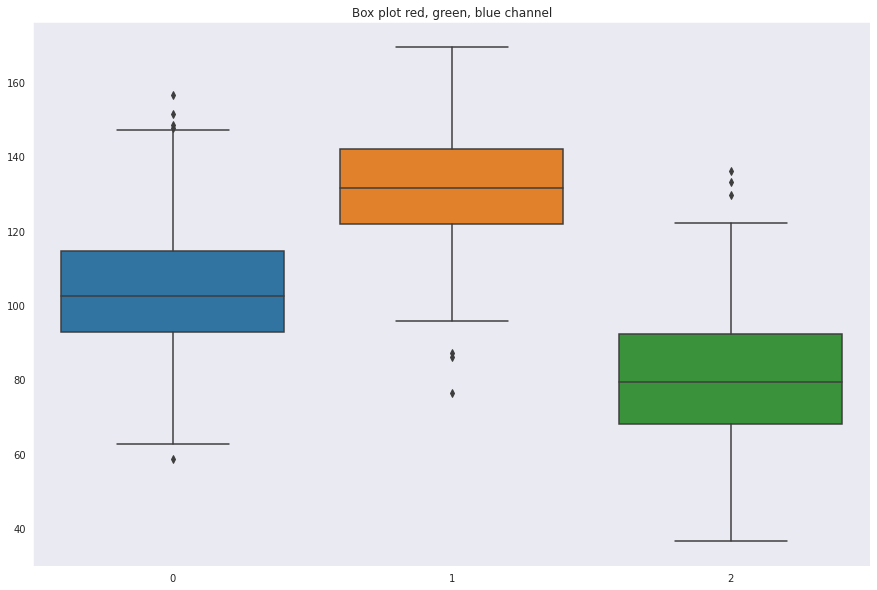
\includegraphics[width=1\linewidth]{images/boxplot_channels_distribution.png}
		\caption{So sánh những kênh màu}
		\label{fig:writing-thesis}
	\end{figure}
	\subsection{4.3 Trực quan hóa mục tiêu}
	\begin{figure}[H]
		\centering
		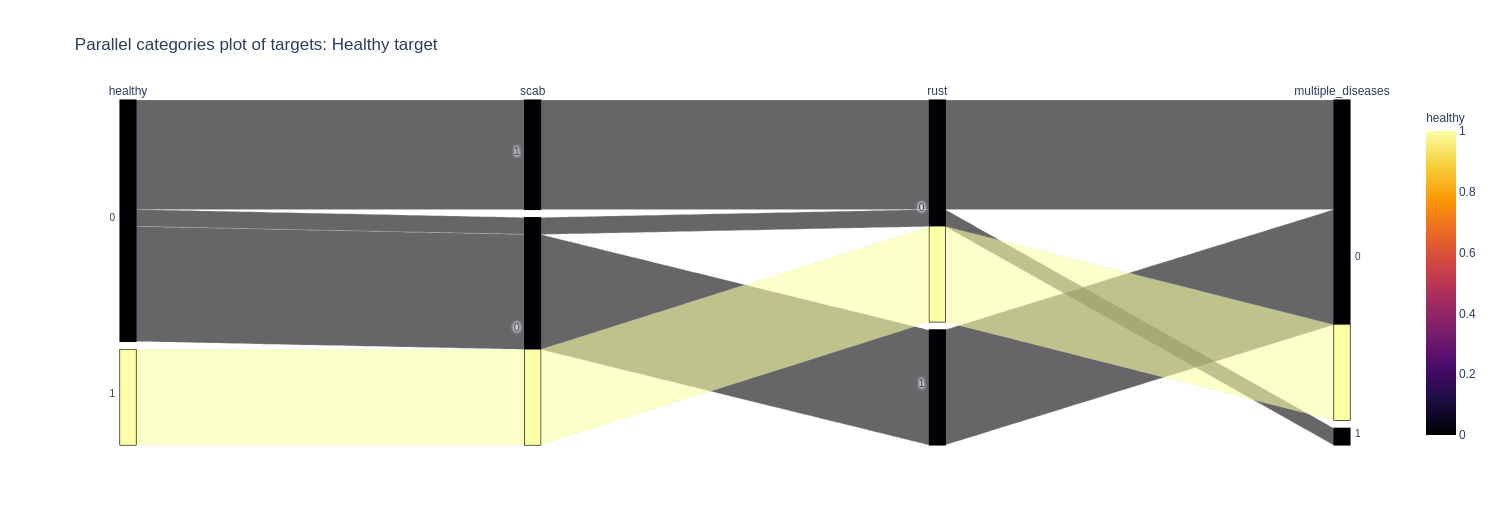
\includegraphics[width=1\linewidth]{images/parallel_categories_healthy_target.png}
		\caption{Biểu đồ loại song song - highlight Healthy Category}
		\label{fig:writing-thesis}
	\end{figure}
	\begin{figure}[H]
		\centering
		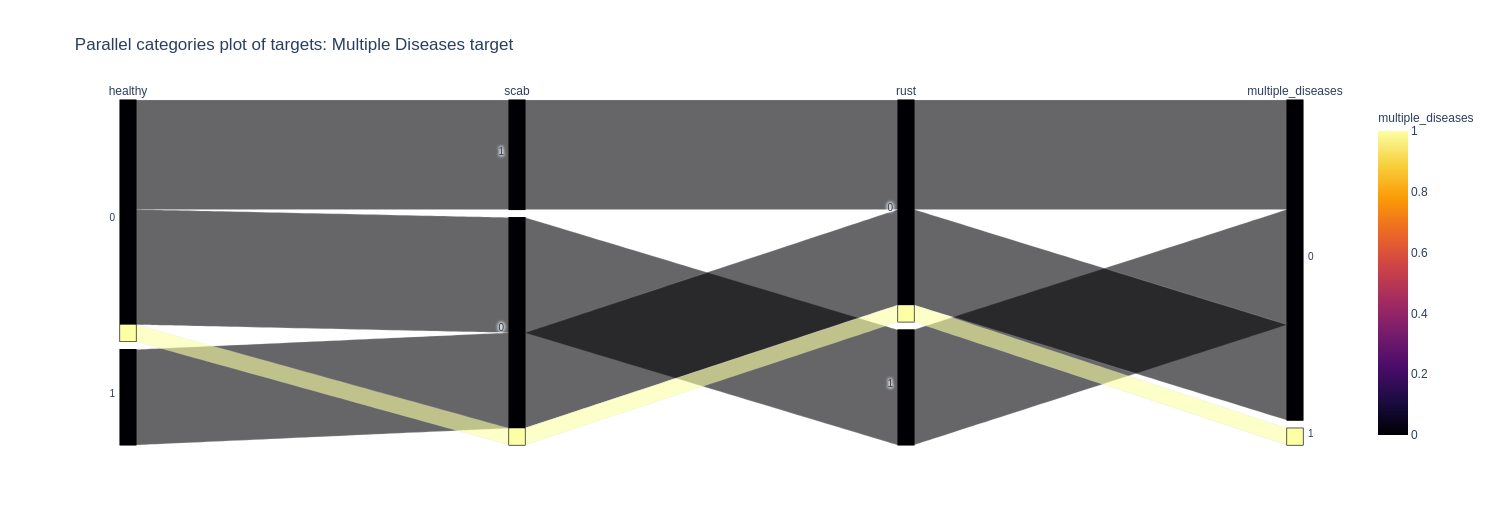
\includegraphics[width=1\linewidth]{images/parallel_categories_multiple_deseases.png}
		\caption{Biểu đồ loại song song - highlight Multiple Diseases Category}
		\label{fig:writing-thesis}
	\end{figure}
	\begin{figure}[H]
		\centering
		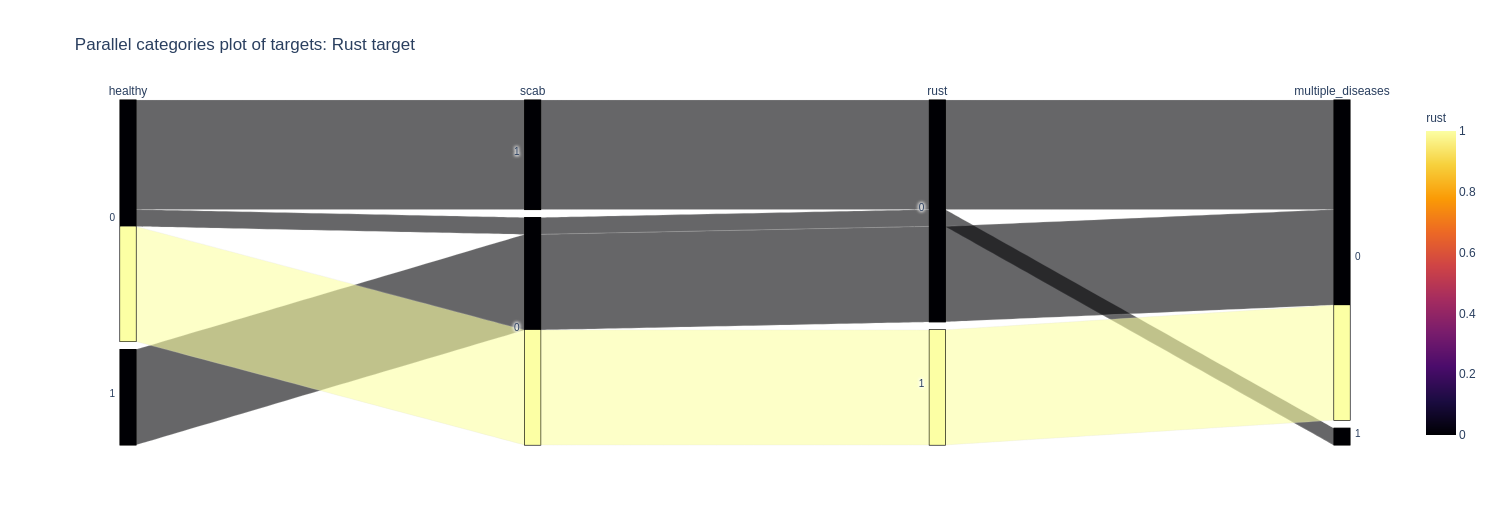
\includegraphics[width=1\linewidth]{images/parallel_categories_rust_target.png}
		\caption{Biểu đồ loại song song - highlight Rust Category}
		\label{fig:writing-thesis}
	\end{figure}
	\begin{figure}[H]
		\centering
		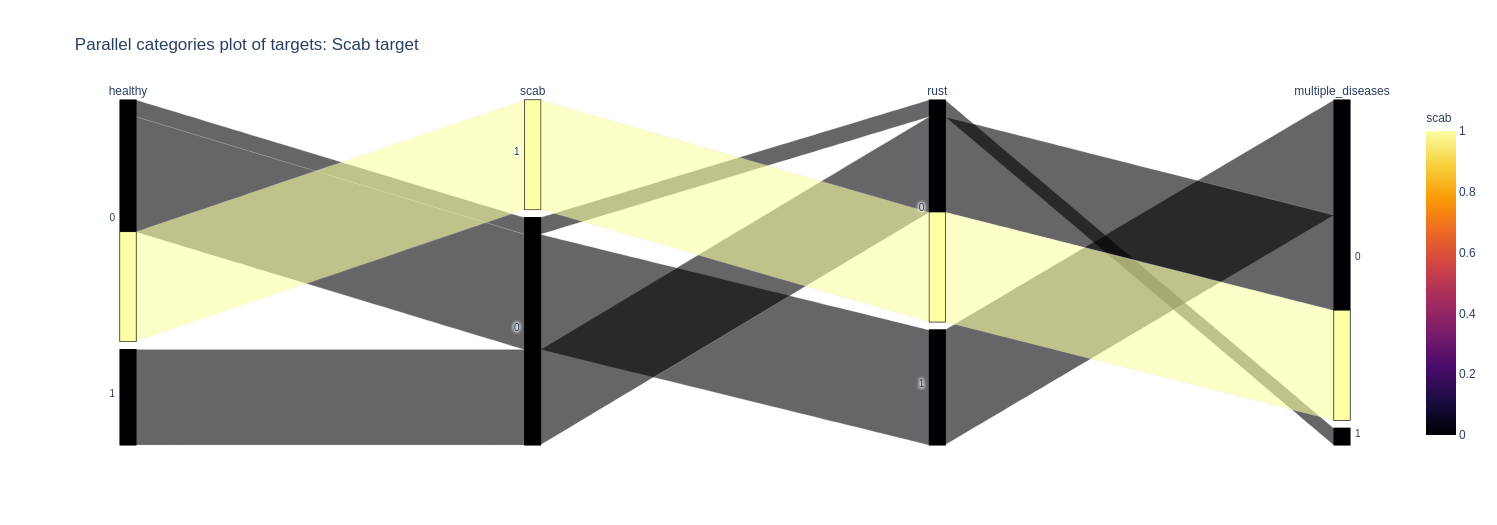
\includegraphics[width=1\linewidth]{images/parallel_categories_scab_target.png}
		\caption{Biểu đồ loại song song - highlight Scab Category}
		\label{fig:writing-thesis}
	\end{figure}
	\begin{figure}[H]
		\centering
		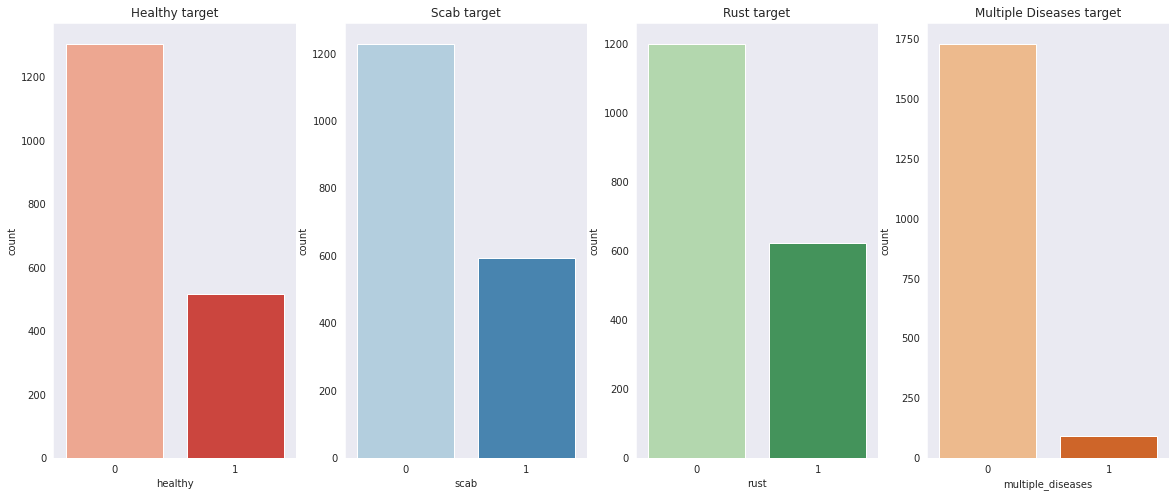
\includegraphics[width=1\linewidth]{images/counting_plot_target.png}
		\caption{Đếm số lượng Healthy - Multiple Diseases - Rust - Scab}
		\label{fig:writing-thesis}
	\end{figure}
	Trực quan hóa mục tiêu phân loại, ta thấy có 32.5\% số lượng lá bị nhiễm scab, 34.2\% số lá bị nhiễm rust, 28.3\% số lá là có sức khỏe tốt, còn lại 5.0\% số lá bị nhiễm bệnh tổng hợp.
	\begin{figure}[H]
		\centering
		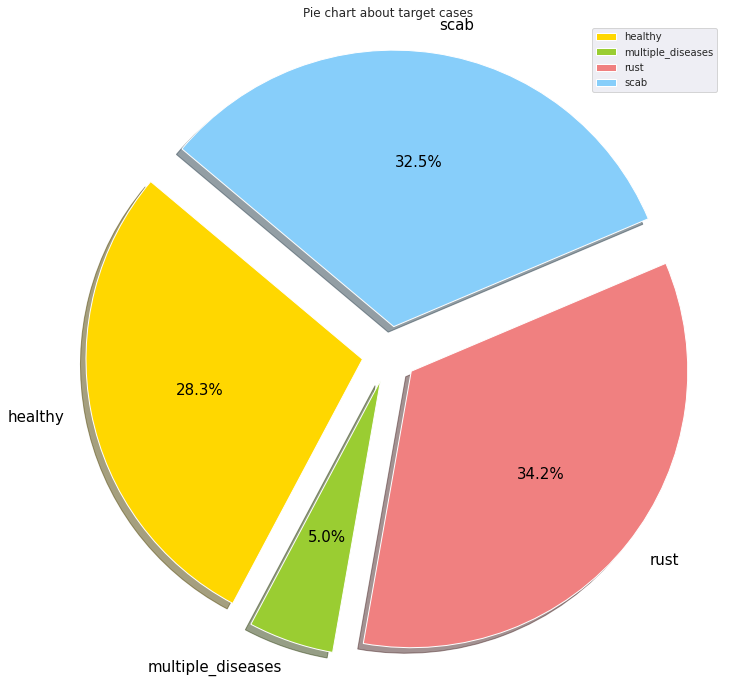
\includegraphics[width=.75\linewidth]{images/pie_chart_targer_plot.png}
		\caption{Biểu đồ phần trăm tỉ lệ các loại bệnh}
		\label{fig:writing-thesis}
	\end{figure}
	\section{5. Xử lý và tăng cường hình ảnh}
	\subsection{5.1 Xác định biên cạnh bằng Canny - The Canny Edge Detection}
	Giải thuật Canny gồm các bước như sau:
	\begin{itemize}
		\item Smooth with gaussian filter - Giảm nhiễm bằng bộ lọc Gaussian
		\begin{itemize}
			\item Tích chập hình ảnh đầu vào với hạt nhân Gaussian để loại bỏ nhiễu tần số cao. Nó rất hữu ích để loại bỏ các kết cấu quy mô nhỏ một cách hiệu quả. Bởi vì Gaussian Kernel có thể phân tách được, nên ta có thể sử dụng phép tích chập phân tách 2D để tính toán nhanh hơn.
		\end{itemize}
		\item Compute h/v gradients. - Tìm đạo hàm mật độ của ảnh
		\begin{itemize}
			\item Gradient là các dẫn xuất bậc nhất của ảnh cho mỗi hướng. Đó là khả năng phát hiện thô của tất cả các cạnh mờ trong hình ảnh và các cạnh trông dày. Vì vậy, chúng ta cần thuật toán làm mỏng để tìm các đường cạnh 1 pixel, đó là Non-Maximal Suppression. Gradient có thể được tính bằng cách sử dụng sự khác biệt trung tâm:
			\begin{align*}
				\text{deltaX}(x,y) = [(x+1, y) - (x-1, y)] / 2 \\
				\text{deltaY}(x,y) = [(x, y+1) - (x, y-1)] / 2
			\end{align*}
		\end{itemize}
		\item Compute magnitude of gradient - Tính giá trị độ lớn của đạo hàm
		\begin{itemize}
			\item Độ lớn của gradient ngang và dọc được sử dụng cho quá trình triệt tiêu không cực đại. Độ lớn có thể được tính bằng
			\begin{align*}
				\text{magnitude} = \sqrt{\text{deltaX}*\text{deltaX} + \text{deltaY}*\text{deltaY}}
			\end{align*}
		\end{itemize}
		\item Perform Non-Maximal Suppression - Thực hiện Non-Maximal Suppression loại bỏ những thành phần dư thừa
		\begin{itemize}
			\item NMS là một thuật toán làm mỏng cạnh. Quá trình này dẫn đến các đường gờ rộng một pixel từ các cạnh dày. Nó yêu cầu h / v gradient và độ lớn của gradient. Ý tưởng cơ bản của NMS là: Nếu một giá trị pixel không lớn hơn các pixel lân cận của nó, thì pixel đó không phải là cạnh (giá trị vô hướng của pixel được đặt bằng 0). Trong quá trình này, nó cũng cần biết hướng của các vectơ gradient để tìm 2 pixel lân cận trên cùng một hướng, sau đó so sánh chúng với pixel hiện tại. (chủ yếu là 4 hoặc 8 hướng là bắt buộc)
		\end{itemize}
		\item Perform Hysteresis Threshold - Phân ngưỡng threshold
		\begin{itemize}
			\item Hysteresis Threshold được sử dụng để loại bỏ các cạnh yếu và cộng, nối các cạnh đã tách. Để kết nối các cạnh, bắt đầu từ pixel lớn hơn ngưỡng cao và tìm kiếm tất cả 8 hàng xóm xung quanh. Nếu hàng xóm lớn hơn ngưỡng thấp, thì nó cũng sẽ trở thành một cạnh. Phạm vi của ngưỡng là:
			\begin{align*}
				0 < \text{low} < \text{high} < 1
			\end{align*}
		\end{itemize}
	\end{itemize}
	\begin{python}
		def canny_edge_detection(image_path, low_threshold=100, high_threshold=200, figsize=(30, 20)):
			# Read image from image_path
			image = io.imread(image_path)
			
			# copy from image to embed image
			embed_image = image.copy()
			
			# Apply Canny Edges Detection with low_threshold and high_threshold
			canny_edges = cv.Canny(image, low_threshold, high_threshold)
			edge_coors = []
			for i in range(canny_edges.shape[0]):
				for j in range(canny_edges.shape[1]):
					if canny_edges[i][j] != 0:
						edge_coors.append((i, j))
			
			# Bounding box detection
			# (row_min, row_min) -> (col_min, col_maxn)
			embed_image[edge_coors[np.argsort([coor[0] for coor in edge_coors])[0]][0]-10:edge_coors[np.argsort([coor[0] for coor in edge_coors])[0]][0]+10, edge_coors[np.argsort([coor[1] for coor in edge_coors])[0]][1]:edge_coors[np.argsort([coor[1] for coor in edge_coors])[-1]][1]] = [255, 0, 0]
			
			# (row_max, row_max) -> (col_min, col_max)
			embed_image[edge_coors[np.argsort([coor[0] for coor in edge_coors])[-1]][0]-10:edge_coors[np.argsort([coor[0] for coor in edge_coors])[-1]][0]+10, edge_coors[np.argsort([coor[1] for coor in edge_coors])[0]][1]:edge_coors[np.argsort([coor[1] for coor in edge_coors])[-1]][1]] = [255, 0, 0]
			
			# (row_min, row_max) -> (col_min, col_min)
			embed_image[edge_coors[np.argsort([coor[0] for coor in edge_coors])[0]][0]:edge_coors[np.argsort([coor[0] for coor in edge_coors])[-1]][0], edge_coors[np.argsort([coor[1] for coor in edge_coors])[0]][1]-10: edge_coors[np.argsort([coor[1] for coor in edge_coors])[0]][1]+10] = [255, 0, 0]
			
			# (row_min, row_max) -> (col_max, col_max)
			embed_image[edge_coors[np.argsort([coor[0] for coor in edge_coors])[0]][0]:edge_coors[np.argsort([coor[0] for coor in edge_coors])[-1]][0], edge_coors[np.argsort([coor[1] for coor in edge_coors])[-1]][1]-10:edge_coors[np.argsort([coor[1] for coor in edge_coors])[-1]][1]+10] = [255, 0, 0]
		
			# Show result
			fig, ax = plt.subplots(nrows=1, ncols=3, figsize=figsize)
			ax[0].imshow(image, cmap='gray')
			ax[0].set_title('Original Image', fontsize=24)
			ax[1].imshow(canny_edges, cmap='gray')
			ax[1].set_title('Canny Edges', fontsize=24)
			ax[2].imshow(embed_image, cmap='gray')
			ax[2].set_title('Bounding Box', fontsize=24)
			plt.show()
	\end{python}
	\begin{figure}[H]
		\centering
		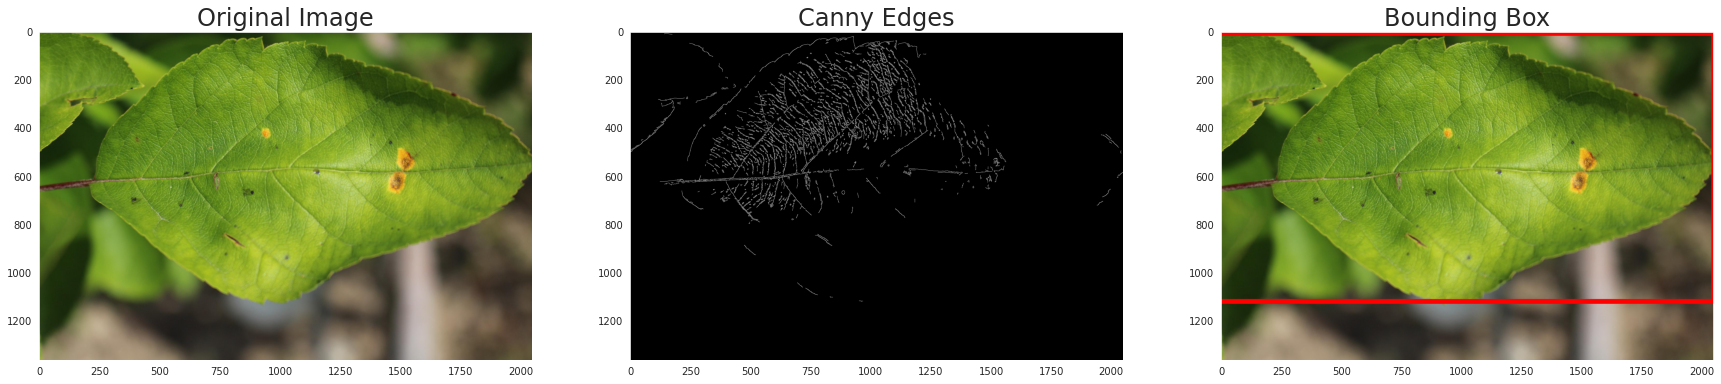
\includegraphics[width=1\linewidth]{images/canny_edge_detector.png}
		\caption{Kết quả giải thuật Canny trên một ảnh ngẫu nhiên}
		\label{fig:writing-thesis}
	\end{figure}
	\begin{figure}[H]
		\centering
		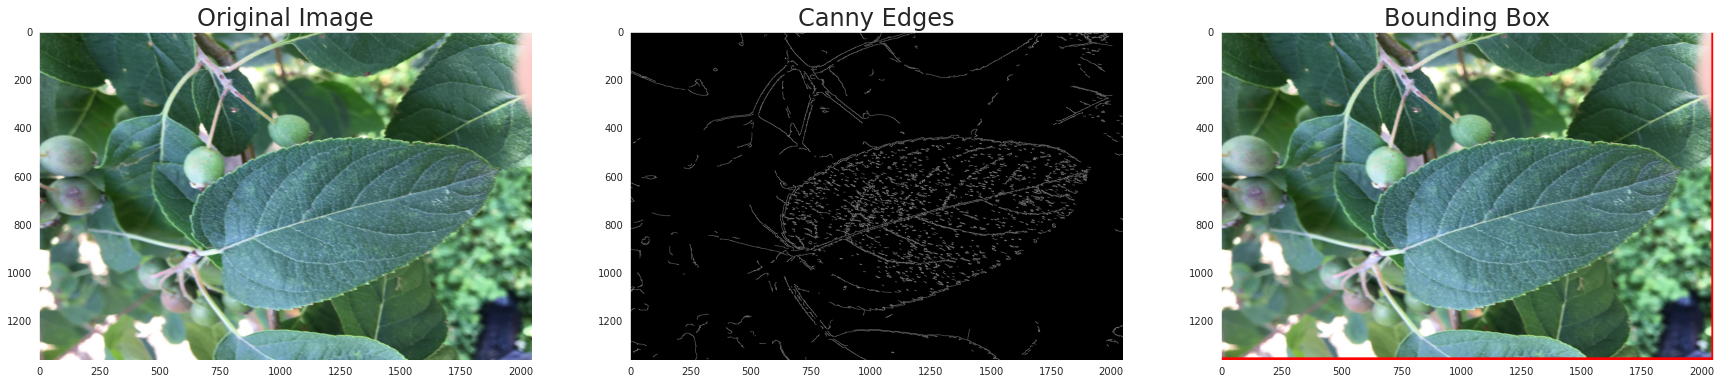
\includegraphics[width=1\linewidth]{images/canny_edge_detector_1.png}
		\caption{Kết quả giải thuật Canny trên một ảnh ngẫu nhiên}
		\label{fig:writing-thesis}
	\end{figure}
	\begin{figure}[H]
		\centering
		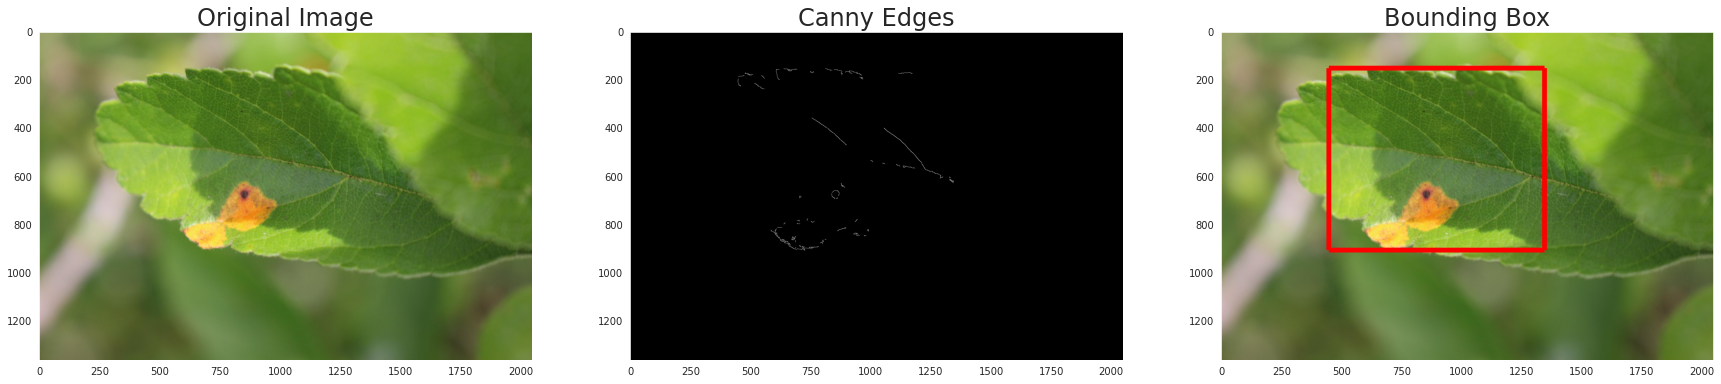
\includegraphics[width=1\linewidth]{images/canny_edge_detector_2.png}
		\caption{Kết quả giải thuật Canny trên một ảnh ngẫu nhiên}
		\label{fig:writing-thesis}
	\end{figure}
	\subsection{5.2 Phép biến đổi lật ảnh - Flipping image}
	Phép lật ảnh là một phép biến đổi đơn giản liên quan đến việc chuyển đổi chỉ mục trên các kênh hình ảnh. Trong lật dọc, thứ tự của các hàng được hoán đổi, trong khi lật dọc, thứ tự của các hàng được hoán đổi.
	\begin{gather*}
	I = A_{ijk}\\
	\text{Horizontal flip}: A_{ijk} \rightarrow A_{i(n+1-j)k}\\
	\text{Vertical flip}: A_{ijk} \rightarrow A_{(m+1-i)jk}
	\end{gather*}
	\begin{python}
		def flipping_image(image_path, figsize=(30, 20)):
			# Read image from image_path
			image = io.imread(image_path)
			
			# Plotting result when applying cv.flip()
			fig, ax = plt.subplots(nrows=1, ncols=3, figsize=figsize)
			ax[0].imshow(image)
			ax[0].set_title('Original Image', fontsize=24)
			ax[1].imshow(cv.flip(image, 0))
			ax[1].set_title('Vertical Flip', fontsize=24)
			ax[2].imshow(cv.flip(image, 1))
			ax[2].set_title('Horizontal Flip', fontsize=24)
			plt.show()
	\end{python}
	\begin{figure}[H]
		\centering
		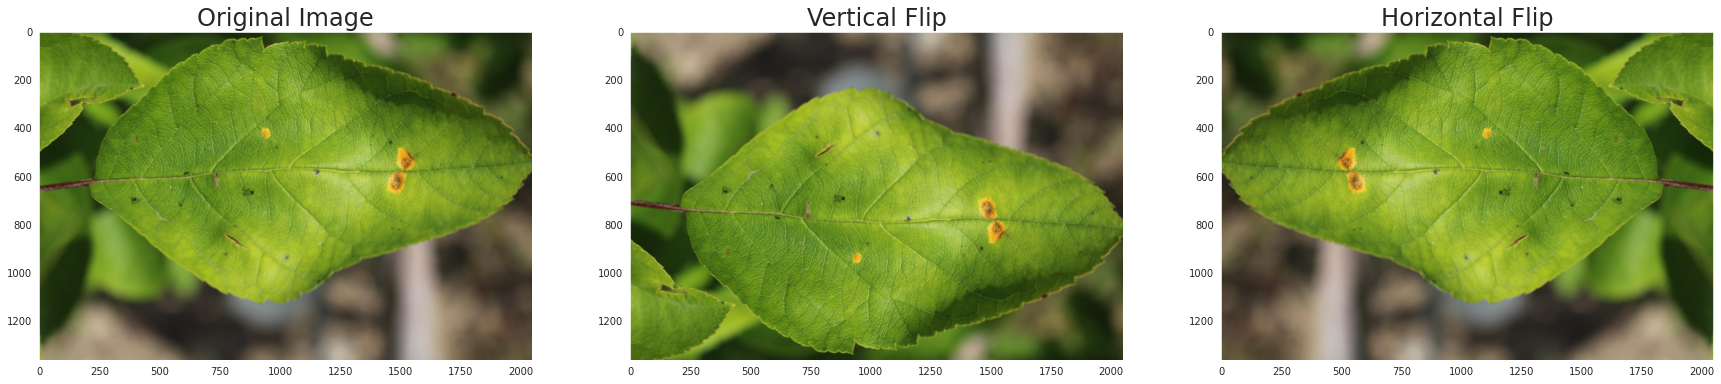
\includegraphics[width=1\linewidth]{images/flipping_image.png}
		\caption{Kết quả phép lật ảnh trên một ảnh ngẫu nhiên}
		\label{fig:writing-thesis}
	\end{figure}
	\begin{figure}[H]
		\centering
		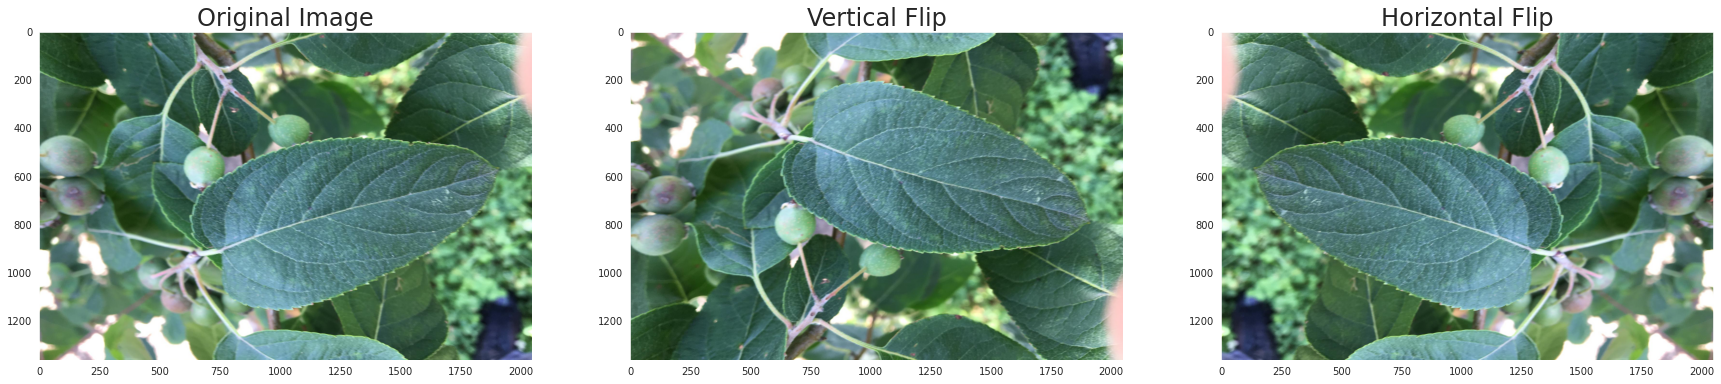
\includegraphics[width=1\linewidth]{images/flipping_image_1.png}
		\caption{Kết quả phép lật ảnh trên một ảnh ngẫu nhiên}
		\label{fig:writing-thesis}
	\end{figure}
	\begin{figure}[H]
		\centering
		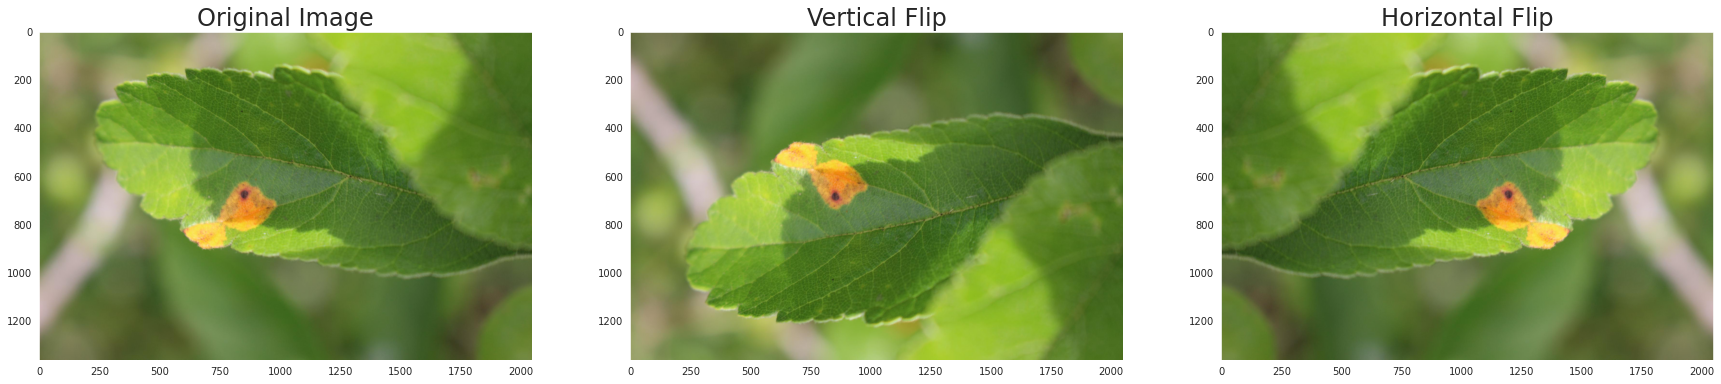
\includegraphics[width=1\linewidth]{images/flipping_image_2.png}
		\caption{Kết quả phép lật ảnh trên một ảnh ngẫu nhiên}
		\label{fig:writing-thesis}
	\end{figure}
	\subsection{5.3 Phép tích chập trên ảnh - Convolutional}
	\begin{figure}[H]
		\centering
		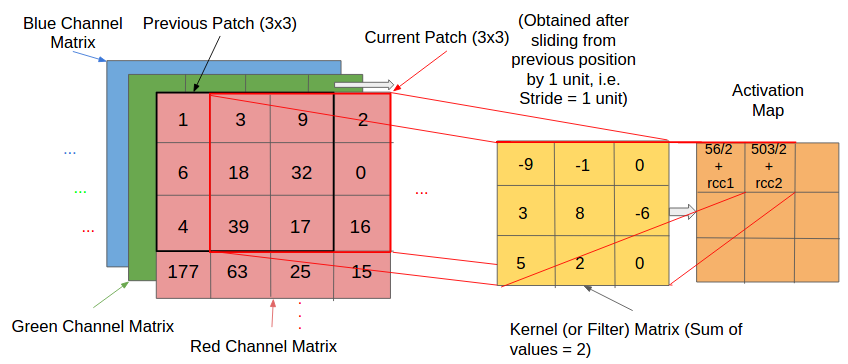
\includegraphics[width=1\linewidth]{architecture/convolution.png}
		\caption{Minh họa Convolutional}
		\label{fig:writing-thesis}
	\end{figure}
	Công thức của phép tích chập trên ảnh
	\begin{align*}
	\text{Conv}(f, h) = \sum_{j}\sum_{k}h_{jk}.f_{(m-j)(n-k)}
	\end{align*}
	\begin{python}
		def convolution(image_path, kernel=np.ones((7, 7), np.float32)/25, figsize=(20, 20)):
			# Read image from image_path
			image = io.imread(image_path)
			
			# Initialization figure image
			fig, ax = plt.subplots(nrows=1, ncols=2, figsize=figsize)
			
			# Apply cv filter 2D with kernel with default 7 x 7 Gaussian
			conv = cv.filter2D(image, -1, kernel)
			
			# Plotting result
			ax[0].imshow(image)
			ax[0].set_title('Original Image', fontsize=24)
			ax[1].imshow(conv)
			ax[1].set_title('Convolved Image', fontsize=24)
			plt.show()
	\end{python}
	\begin{figure}[H]
		\centering
		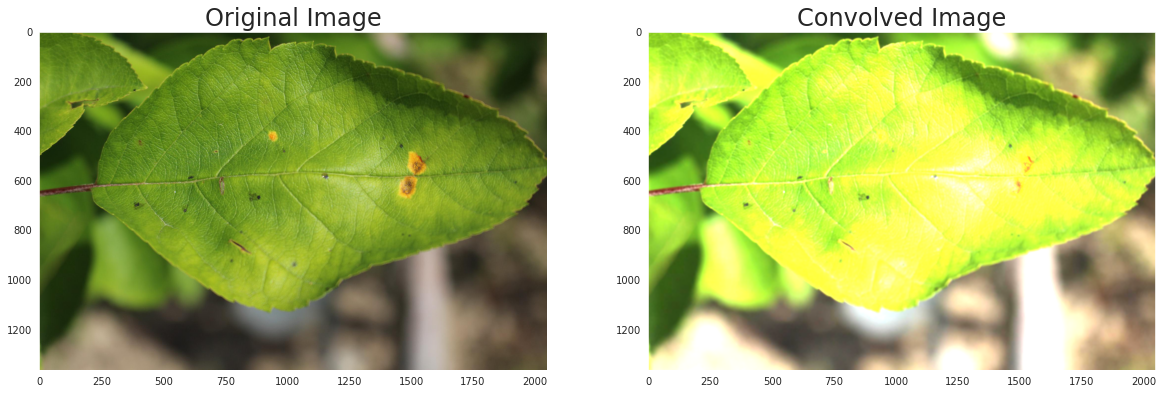
\includegraphics[width=1\linewidth]{images/conv.png}
		\caption{Kết quả phép tích chập trên một ảnh ngẫu nhiên}
		\label{fig:writing-thesis}
	\end{figure}
	\begin{figure}[H]
		\centering
		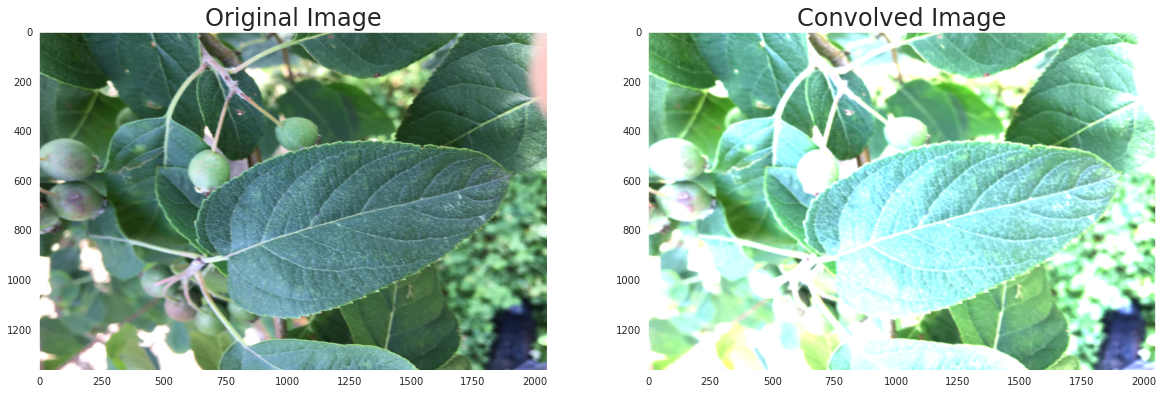
\includegraphics[width=1\linewidth]{images/conv_1.png}
		\caption{Kết quả phép tích chập trên một ảnh ngẫu nhiên}
		\label{fig:writing-thesis}
	\end{figure}
	\begin{figure}[H]
		\centering
		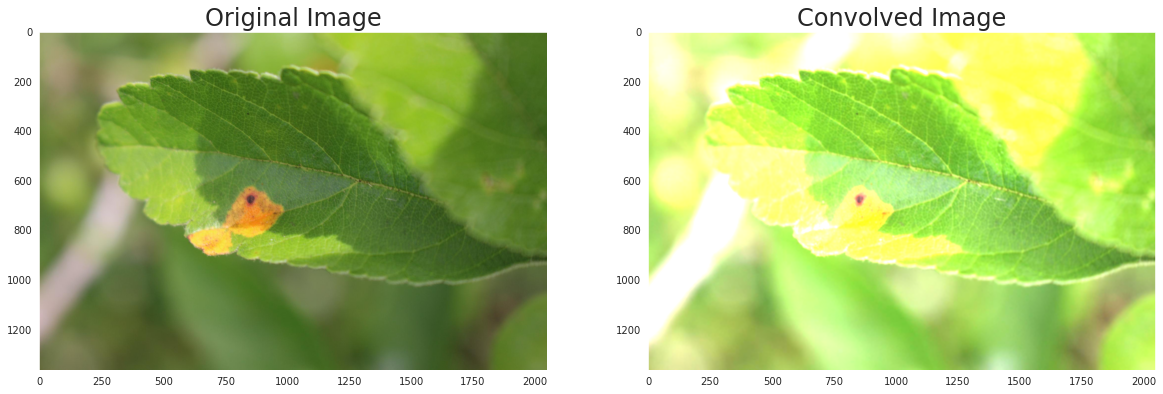
\includegraphics[width=1\linewidth]{images/conv_2.png}
		\caption{Kết quả phép tích chập trên một ảnh ngẫu nhiên}
		\label{fig:writing-thesis}
	\end{figure}
	\subsection{5.4 Làm trơn ảnh - Bluring image}
	\begin{python}
		def blur_image(image_path, kernel_width=100, kernel_height=100, figsize=(20, 20)):
			# Read image from image_path
			image = io.imread(image_path)
			
			# Initialization figure image
			fig, ax = plt.subplots(nrows=1, ncols=2, figsize=figsize)
			
			# Plotting result when applying cv.blur()
			ax[0].imshow(image)
			ax[0].set_title('Original Image', fontsize=24)
			ax[1].imshow(cv.blur(image, (kernel_width, kernel_height)))
			ax[1].set_title('Blurred Image', fontsize=24)
			plt.show()
	\end{python}
	\begin{figure}[H]
		\centering
		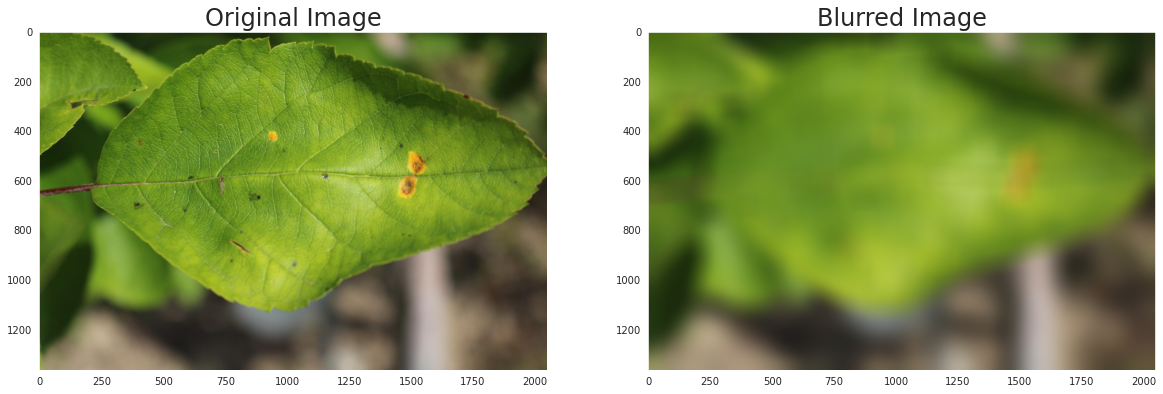
\includegraphics[width=1\linewidth]{images/blur_1.png}
		\caption{Kết quả phép làm trơn ảnh trên một ảnh ngẫu nhiên}
		\label{fig:writing-thesis}
	\end{figure}
	\begin{figure}[H]
		\centering
		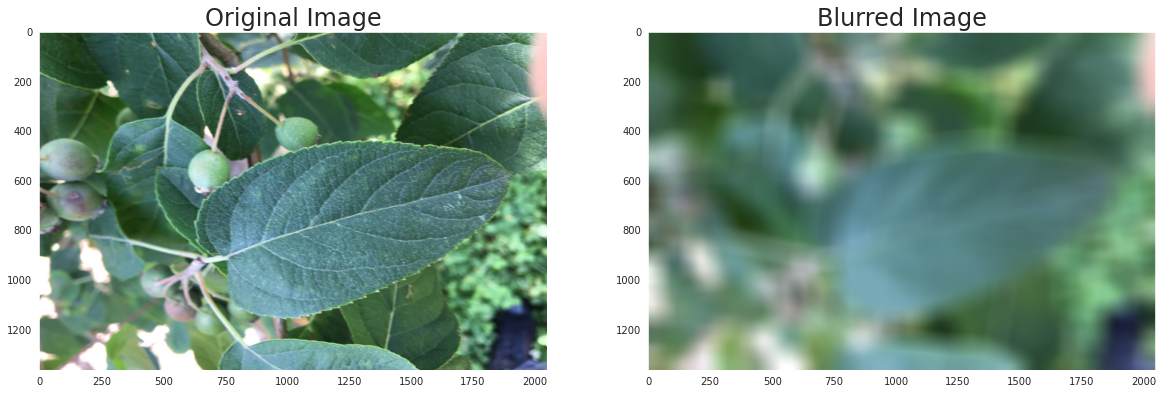
\includegraphics[width=1\linewidth]{images/blur_2.png}
		\caption{Kết quả phép làm trơn ảnh trên một ảnh ngẫu nhiên}
		\label{fig:writing-thesis}
	\end{figure}
	\begin{figure}[H]
		\centering
		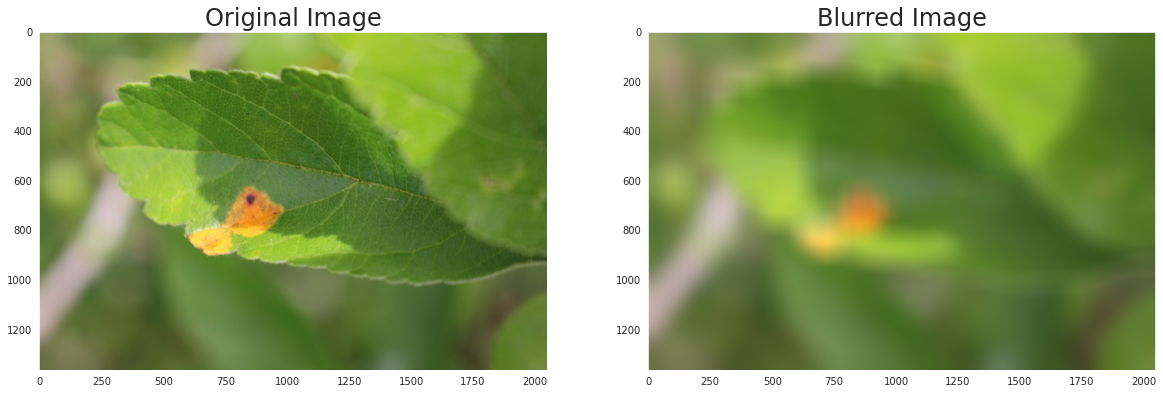
\includegraphics[width=1\linewidth]{images/blur_3.png}
		\caption{Kết quả phép làm trơn ảnh trên một ảnh ngẫu nhiên}
		\label{fig:writing-thesis}
	\end{figure}
	\section{6. Cài đặt Neural Networks}
	\subsection{6.1 Cài đặt các thư viện hỗ trợ}
	\begin{python}
		!pip install pretrainedmodels
		!pip install albumentations==0.4.5
	\end{python}
	\subsection{6.2 Tải dữ liệu}
	Sử dụng package gdown để download dữ liệu 
	\begin{python}
		# https://drive.google.com/file/d/1jfkX_NXF8shxyWZCxJkzsLPDr4ebvdOP/view?usp=sharing
		!pip install gdown
		!gdown https://drive.google.com/uc?id=1jfkX_NXF8shxyWZCxJkzsLPDr4ebvdOP
		!unzip -q plant-pathology-2020-fgvc7.zip -d /content/plant-pathology-2020-fgvc7
		!rm plant-pathology-2020-fgvc7.zip
	\end{python}
	\subsection{6.3 Cài đặt các thông số}
	Với những mạng khác nhau, chúng ta cần điều chỉnh BATCH\_SIZE cho hợp lý
	\begin{itemize}
		\item ResNet18, BATCH\_SIZE = 32
		\item ResNet34, BATCH\_SIZE = 24
		\item ResNet50, BATCH\_SIZE = 16
		\item Efficient-B5, BATCH\_SIZE = 2
	\end{itemize}
	\subsection{6.4 Định nghĩa cấu trúc tập dữ liệu}
	\begin{python}
		class PlantDataset(Dataset):
		
			def __init__(self, df, transforms=None):
				self.df = df
				self.transforms=transforms
		
			def __len__(self):
				return self.df.shape[0]
		
			def __getitem__(self, idx):
				# Solution 01: Read from raw image
				image_src = IMAGES_PATH + self.df.loc[idx, 'image_id'] + '.jpg'
		
				# Solution 02: Read from npy file, we convert all images in images folder from .jpg to .npy
				# image_src = np.load(IMAGES_PATH + self.df.loc[idx, 'image_id'] + '.npy')
		
				# print(image_src)
				image = cv.imread(image_src, cv.IMREAD_COLOR)
				if image.shape != IMG_SHAPE:
					image = image.transpose(1, 0, 2)
				image = cv.cvtColor(image, cv.COLOR_BGR2RGB)
				labels = self.df.loc[idx, ['healthy', 'multiple_diseases', 'rust', 'scab']].values
				labels = torch.from_numpy(labels.astype(np.int8))
				labels = labels.unsqueeze(-1)
		
				if self.transforms:
					transformed = self.transforms(image=image)
				image = transformed['image']
		
				return image, labels
	\end{python}
	\subsection{6.5 Tăng cường dữ liệu}
	\begin{python}
		# Train transformation
		transforms_train = A.Compose([
			A.RandomResizedCrop(height=SIZE, width=SIZE, p=1.0),
			A.OneOf([A.RandomBrightness(limit=0.1, p=1), A.RandomContrast(limit=0.1, p=1)]),
			A.OneOf([A.MotionBlur(blur_limit=3), A.MedianBlur(blur_limit=3), A.GaussianBlur(blur_limit=3)], p=0.5),
			A.VerticalFlip(p=0.5),
			A.HorizontalFlip(p=0.5),
			A.ShiftScaleRotate(
			shift_limit=0.2,
			scale_limit=0.2,
			rotate_limit=20,
			interpolation=cv.INTER_LINEAR,
			border_mode=cv.BORDER_REFLECT_101,
			p=1,
		),
			A.Normalize(mean=(0.485, 0.456, 0.406), std=(0.229, 0.224, 0.225), max_pixel_value=255.0, p=1.0),
			A.pytorch.ToTensorV2(p=1.0),
		], p=1.0)
		
		# Validation transformation
		transforms_valid = A.Compose([
			A.Resize(height=SIZE, width=SIZE, p=1.0),
			A.Normalize(mean=(0.485, 0.456, 0.406), std=(0.229, 0.224, 0.225), max_pixel_value=255.0, p=1.0),
			A.pytorch.ToTensorV2(p=1.0),
		])
	\end{python}
	\subsection{6.6 Stratified K-Folds}
	Thực thi Stratified K-Folds
	\begin{python}
		# Get label from df_train
		train_labels = df_train.iloc[:, 1:].values
		train_y = train_labels[:, 2] + train_labels[:, 3] * 2 + train_labels[:, 1] * 3
		
		folds = StratifiedKFold(n_splits=N_FOLDS, shuffle=True, random_state=SEED)
		oof_preds = np.zeros((df_train.shape[0], 4))
	\end{python}
	Cross-validation là một quy trình lấy mẫu lại được sử dụng để đánh giá các mô hình Máy Học trên một mẫu dữ liệu hạn chế.
	
	Thủ tục có một tham số duy nhất được gọi là $K$ đề cập đến số lượng nhóm mà một mẫu dữ liệu nhất định sẽ được chia thành. Do đó, thủ tục này thường được gọi là k-fold cross-validation. Khi một giá trị cụ thể cho k được chọn, nó có thể được sử dụng thay cho $K$ trong tham chiếu đến mô hình, chẳng hạn như $K = 10$ trở thành 10-fold cross-validation.
	
	Các bước bước thủ tục $K$-Fold Cross-Validation
	\begin{enumerate}
		\item Xáo trộn tập dữ liệu một cách ngẫu nhiên.
		\item Chia tập dữ liệu thành $K$ nhóm
		\item Với mỗi nhóm:
		\begin{enumerate}
			\item Lấy nhóm làm tập dữ liệu thử nghiệm (test data set) hoặc làm tập Holdout
			\item Lấy các nhóm còn lại làm tập dữ liệu huấn luyện
			\item Khớp một mô hình vào tập huấn luyện và đánh giá mô hình đó trên tập thử nghiệm
			\item Giữ lại điểm đánh giá và loại bỏ mô hình
		\end{enumerate}
		\item Tổng hợp kết quả của mô hình bằng cách sử dụng mẫu điểm đánh giá mô hình
	\end{enumerate}
	\textbf{Cách chọn $K$ trong $K$-Fold Cross-Validation}
	Viêc chọn giá trị $K$ phù hợp thường được lược chọn rất cẩn thận
	
	Giá trị $K$ được chọn không tốt có thể dẫn đến ý tưởng đại diện sai về kỹ năng của mô hình, chẳng hạn như điểm có phương sai cao (có thể thay đổi nhiều dựa trên dữ liệu được sử dụng để phù hợp với mô hình) hoặc độ chệch cao (chẳng hạn như đánh giá quá cao khả năng của mô hình).
	
	Ta có ba chiến lược chọn giá trị $K$ như sau:
	\begin{itemize}
		\item Đại diện (Representative): Giá trị của k được chọn sao cho mỗi tập huấn luyện/ thử nghiệm mẫu dữ liệu đủ lớn để đại diện về mặt thống kê cho tập dữ liệu rộng hơn.
		\item $K = 10$: Giá trị của $K$ được cố định thành 10, một giá trị đã được tìm thấy thông qua thử nghiệm thường dẫn đến ước tính kỹ năng mô hình với độ chệch thấp và phương sai khiêm tốn.
		\item $K = n$: Giá trị của $K$ được cố định thành $n$, trong đó $n$ là kích thước của tập dữ liệu để tạo cơ hội cho mỗi mẫu thử nghiệm được sử dụng trong tập dữ liệu chờ. Cách tiếp cận này được gọi là xác thực chéo bỏ qua (leave-one-out cross-validation).
	\end{itemize}
	\subsection{6.7 Định nghĩa custom layer cho pre-trained model}
	
	\subsubsection{6.7.1 ResNet}
	Phần tùy chỉnh layer của ResNet để phù hợp với dữ liệu đang có. Tùy chỉnh khởi tạo mô hình ResNet18, 34 hay 50 bằng câu lệnh torchvision.models.resnet<architecture ResNet>(pretrained=True)
	
	Mô hình nhận đầu vào có kích thước là số đặc trưng của ResNet, kích thước đầu ra là 4 (4 loại bệnh trên lá cây)
	\begin{python}
		# Download pretrained weights.
		model = torchvision.models.resnet34(pretrained=True)
		
		# print number of features
		num_features = model.fc.in_features
		print(num_features)
		
		
		# custome layers
		model.fc = nn.Sequential(
		nn.Linear(num_features, 512), # With bias default = True
		nn.ReLU(),
		nn.BatchNorm1d(512),
		nn.Dropout(0.5), # Drop out 0.5 for avoiding overfitting
		
		nn.Linear(512, 256), # With bias default = True
		nn.ReLU(),
		nn.BatchNorm1d(256),
		nn.Dropout(0.5), # Dropout 0.5 for avoiding overftting
		
		nn.Linear(256, 4)) # With bias default = True
		
		# initialize weights function
		def init_weights(m):
			if type(m) == nn.Linear:
			torch.nn.init.xavier_uniform_(m.weight)
			m.bias.data.fill_(0.01)
		
		# apply model with init weights
		model.apply(init_weights)
		
		# transfer model to device (cuda:0 mean using GPU, xla mean using TPU, otherwise using CPU)
		model = model.to(device)
		
		# Model details
		model
	\end{python}
	\subsubsection{6.7.2 EfficientNet B5}
	\begin{python}
		# Initialization Model EfficientNet B5
		model = EfficientNet.from_pretrained('efficientnet-b5') 
		
		# Take input features size
		num_ftrs = model._fc.in_features
		
		# Custom Model Sequential
		model._fc = nn.Sequential(nn.Linear(num_ftrs,1000,bias=True),
		nn.ReLU(),
		nn.Dropout(p=0.5), # Dropout 0.5 for avoiding overftting
		nn.Linear(1000,4, bias = True)) # Linear model with bias, output size is 4, equal to number of classes diseases leaf
		
		# Connect with device, device is cuda:0 if using GPU, xla if using TPU
		model.to(device)
		
		# Show model details
		model
	\end{python}
	\subsubsection{6.7.3 Cross entropy loss one hot}
	\begin{python}
		# define cross entropy loss one hot
		class CrossEntropyLossOneHot(nn.Module):
			def __init__(self):
				super(CrossEntropyLossOneHot, self).__init__()
				self.log_softmax = nn.LogSoftmax(dim=-1)
		
			def forward(self, preds, labels):
				return torch.mean(torch.sum(-labels * self.log_softmax(preds), -1))
	\end{python}
	\subsubsection{6.7.4 Dense cross entropy}
	\begin{python}
		# define dense cross entropy
		class DenseCrossEntropy(nn.Module):
		
			def __init__(self):
				super(DenseCrossEntropy, self).__init__()
		
		
			def forward(self, logits, labels):
				logits = logits.float()
				labels = labels.float()
		
				logprobs = F.log_softmax(logits, dim=-1)
		
				loss = -labels * logprobs
				loss = loss.sum(-1)
		
				return loss.mean()
	\end{python}
	\section{7. Huấn luyện và đánh giá mô hình Neural Networks}
	\subsection{7.1 Huấn luyện trên 1-Fold}
	Việc huấn luyện trên một fold gồm các bước như sau:
		
	Với mỗi epoch
	\begin{itemize}
		\item Bước 01: Gọi model train
		\item Bước 02: Với mỗi step và batch trong dataloader train
		\begin{itemize}
			\item Chuẩn bị dữ liệu
			\item Forward pass và tính toán độ lỗi
			\item Backward pass
			\item Cập nhật trọng số và làm rỗng gradient .zero\_grad()
		\end{itemize}
		\item Bước 03: Đánh giá mô hình.  Với mỗi step và batch trong dataloader valid
		\begin{itemize}
			\item Chuẩn bị dữ liệu, nhãn
			\item Ngưng kích hoạt tính toán gradient Pytorch và tính toán output từ mô hình
			\item Cập nhật độ lỗi
		\end{itemize}
		\item Bước 04: Tính toán độ lỗi huấn luyện, độ lỗi xác thực và in ra kết quả huấn luyện tại bước thứ epoch
	\end{itemize}
	
	\subsection{7.2 Huấn luyện mô hình Neural Networks}
	Việc huấn luyện mô hình Neural Networks với mạng EfficientNet B5, ResNet được thực hiện bằng vòng lặp với các bước:
	
	Với mỗi fold thứ i, train thứ idx, valid thứ ida:
	\begin{itemize}
		\item Bước 01: Chuẩn bị dữ liệu
		\item Bước 02: Biến đổi dữ liệu và dùng DataLoader Pytorch để tải dữ liệu
		\item Bước 03: Khởi tạo Cross Entropy (Dense Cross-Entropy), Optimizer (AdamW)
		\item Bước 04: Huấn luyện mô hình trên 1-fold
		\item Bước 05: Đánh giá mô hình
		\item Bước 06: Lưu mô hình và tính toán độ chính xác của mô hình
	\end{itemize}
	\section{8. Các kết quả đạt được}
	\subsection{8.1 Kết quả với ResNet18}
	Huấn luyện mô hình với mạng ResNet18, với 5-Fold, mỗi fold gồm 10 epoch
	\begin{figure}[H]
		\centering
		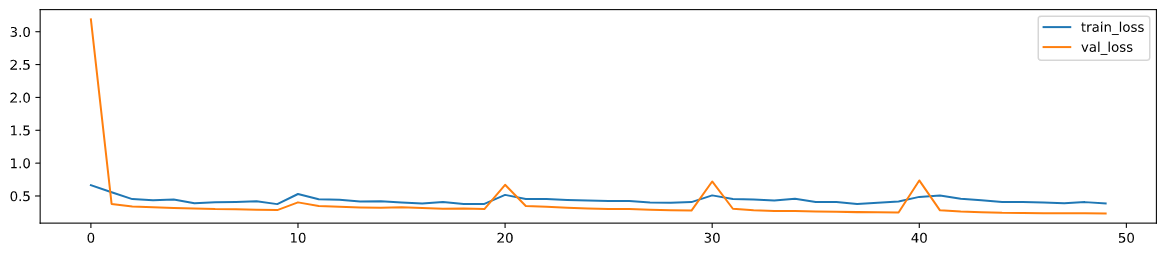
\includegraphics[width=1\linewidth]{results/resnet18/training_loss_results.png}
		\caption{Đồ thị training loss, validation loss ResNet18}
		\label{fig:writing-thesis}
	\end{figure}
	\begin{figure}[H]
		\centering
		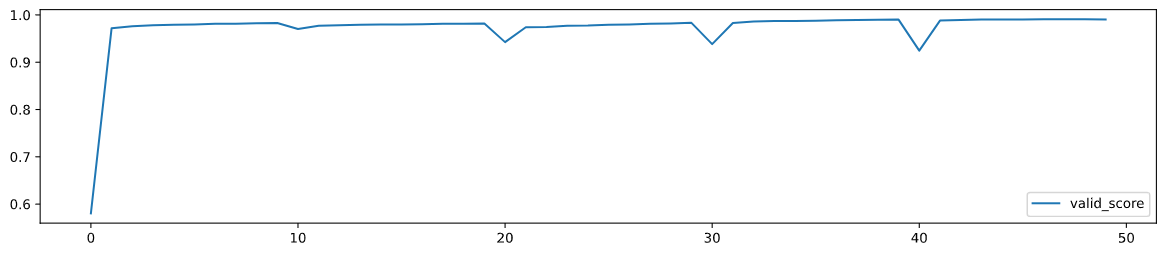
\includegraphics[width=1\linewidth]{results/resnet18/valid_score_results.png}
		\caption{Đồ thị Validation Score ResNet18}
		\label{fig:writing-thesis}
	\end{figure}
	\begin{figure}[H]
		\centering
		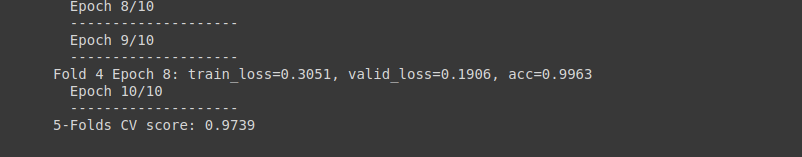
\includegraphics[width=1\linewidth]{results/resnet18/CV_Score_5_Folds_ResNet18.png}
		\caption{Kết quả Cross Validation Score sau 5-Folds Training ResNet18}
		\label{fig:writing-thesis}
	\end{figure}
	\subsection{8.2 Kết quả với ResNet34}
	Huấn luyện mô hình với mạng ResNet34, với 5-Fold, mỗi fold gồm 10 epoch
	\begin{figure}[H]
		\centering
		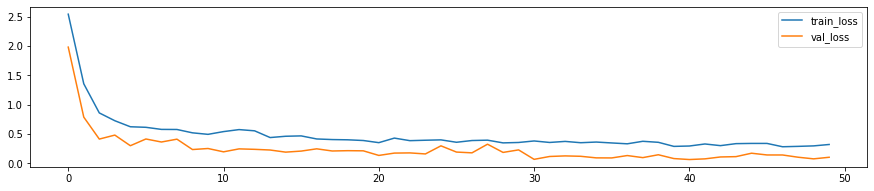
\includegraphics[width=1\linewidth]{results/resnet34/training_loss_results.png}
		\caption{Đồ thị training loss, validation loss ResNet34}
		\label{fig:writing-thesis}
	\end{figure}
	\begin{figure}[H]
		\centering
		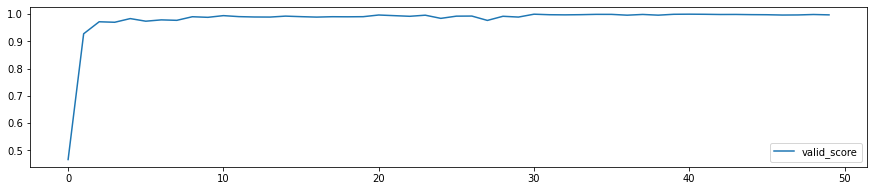
\includegraphics[width=1\linewidth]{results/resnet34/valid_score_results.png}
		\caption{Đồ thị Validation Score ResNet34}
		\label{fig:writing-thesis}
	\end{figure}
	\begin{figure}[H]
		\centering
		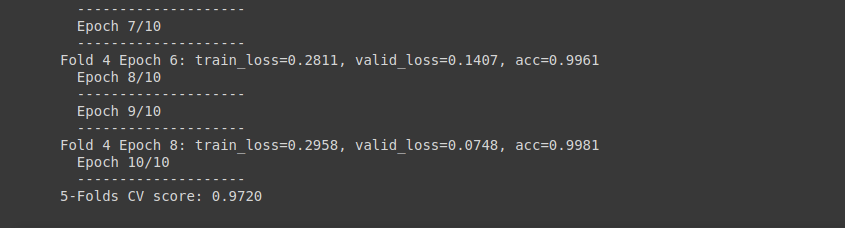
\includegraphics[width=1\linewidth]{results/resnet34/CV_Score_5_Folds_ResNet34.png}
		\caption{Kết quả Cross Validation Score sau 5-Folds Training ResNet34}
		\label{fig:writing-thesis}
	\end{figure}
	\subsection{8.3 Kết quả với ResNet50}
	Huấn luyện mô hình với mạng ResNet50, với 5-Fold, mỗi fold gồm 10 epoch
	\begin{figure}[H]
		\centering
		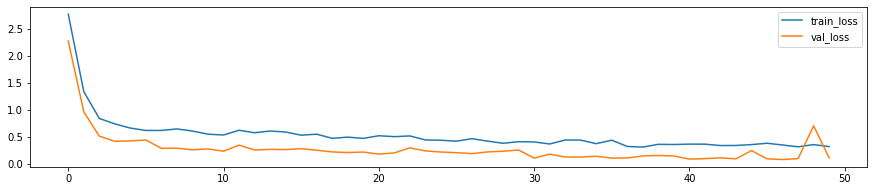
\includegraphics[width=1\linewidth]{results/resnet50/training_loss_results.png}
		\caption{Đồ thị training loss, validation loss ResNet50}
		\label{fig:writing-thesis}
	\end{figure}
	\begin{figure}[H]
		\centering
		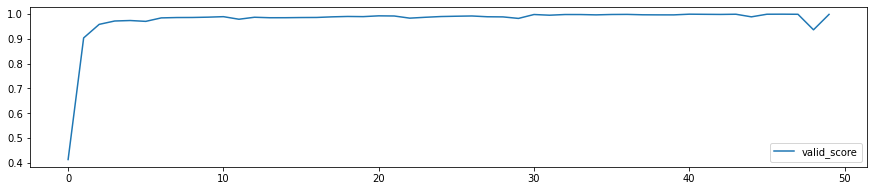
\includegraphics[width=1\linewidth]{results/resnet50/valid_score_results.png}
		\caption{Đồ thị Validation Score ResNet50}
		\label{fig:writing-thesis}
	\end{figure}
	\begin{figure}[H]
		\centering
		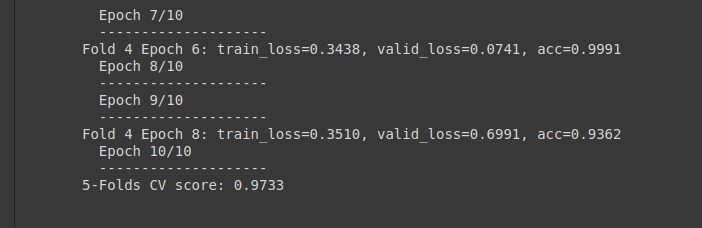
\includegraphics[width=1\linewidth]{results/resnet50/CV_Score_5_Folds_ResNet50.png}
		\caption{Kết quả Cross Validation Score sau 5-Folds Training ResNet50}
		\label{fig:writing-thesis}
	\end{figure}
	\subsection{8.4 Kết quả với EfficientNet B5}
	Huấn luyện mô hình với mạng EfficientNet B5, với 5-Fold, mỗi fold gồm 10 epoch
	\begin{figure}[H]
		\centering
		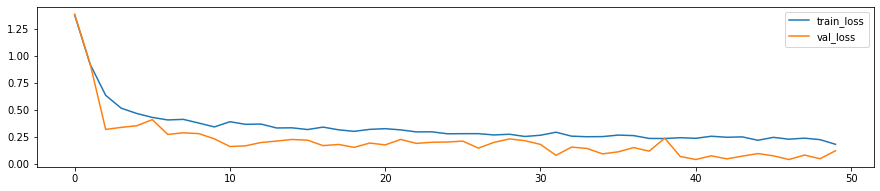
\includegraphics[width=1\linewidth]{results/efficientnet-b5/training_loss_results_50.png}
		\caption{Đồ thị training loss, validation loss EfficientNet B5}
		\label{fig:writing-thesis}
	\end{figure}
	\begin{figure}[H]
		\centering
		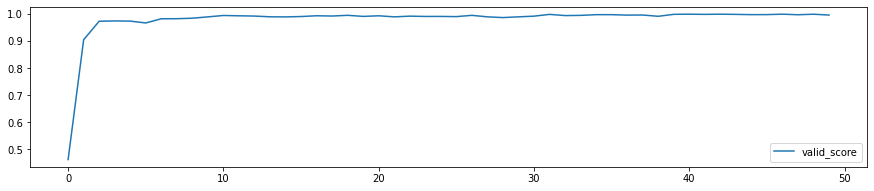
\includegraphics[width=1\linewidth]{results/efficientnet-b5/valid_score_results_50.png}
		\caption{Đồ thị Validation Score EfficientNet B5}
		\label{fig:writing-thesis}
	\end{figure}
	\begin{figure}[H]
		\centering
		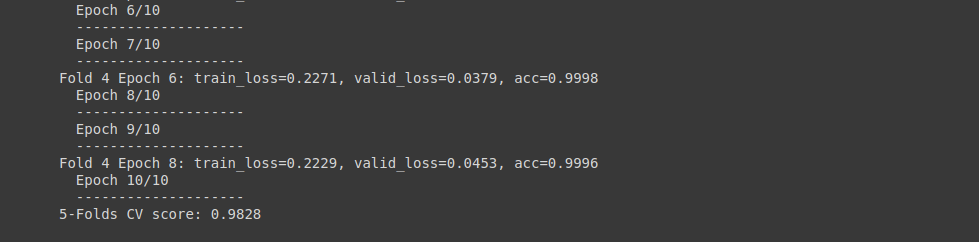
\includegraphics[width=1\linewidth]{results/efficientnet-b5/CV_Score_5_Folds_EfficientNetB5_50.png}
		\caption{Kết quả Cross Validation Score sau 5-Folds Training EfficientNet B5}
		\label{fig:writing-thesis}
	\end{figure}
	\section{9. Kết luận}
	Với phương pháp học Transfer Learning với mạng ResNet18, 34, 50 và EfficentNet B5 đã giải quyết bài toán phân loại lá bệnh một cách tốt với độ chính xác tương đối cao sau 5-Fold là hơn 97\%, với kỹ thuật sử dụng dropout, K-Fold Cross Validation đảm bảo giảm thiểu, tránh overfitting
	
	\begin{center}
		\begin{tabular}{ |c|c|c|c| } 
			\hline
			Neural Nets & K-Fold & Epoch/ Fold & Cross-Validation Score \\ \hline
			ResNet18 & 5 & 10 & 0.9739 \\ 
			ResNet34 & 5 & 10 & 0.9720 \\ 
			ResNet50 & 5 & 10 & 0.9733 \\ 
			EfficientNetB5 & 5 & 10 & 0.9828 \\ 
			\hline
		\end{tabular}
	\end{center}
	Note: Khi tăng epoch huấn luyện EfficientNet B5 lên 20 epoch mỗi fold, kết quả đạt
	\begin{figure}[H]
		\centering
		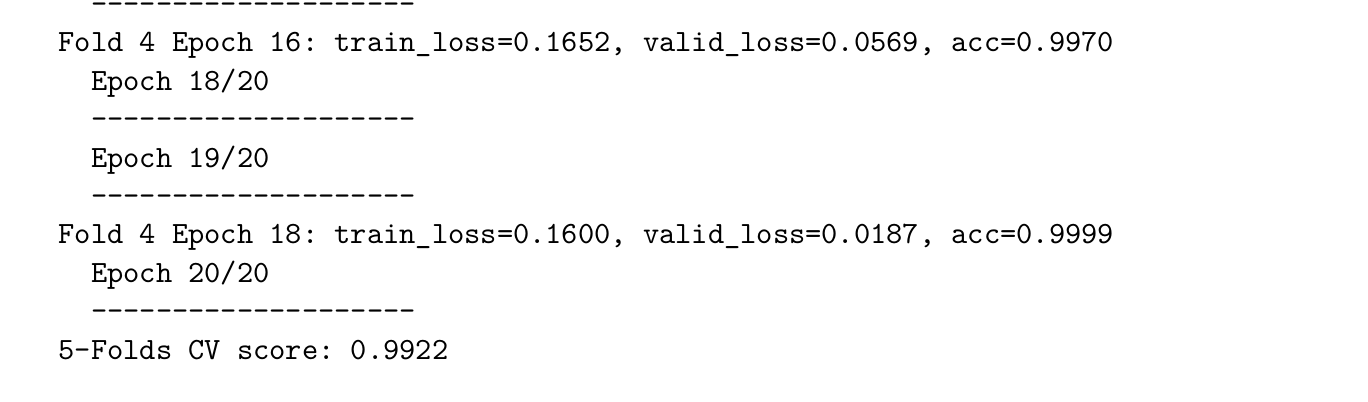
\includegraphics[width=1\linewidth]{results/efficientnet-b5/CV_Score_5_Folds_EfficientNetB5.png}
		\caption{Kết quả Cross Validation Score sau 5-Folds Training}
		\label{fig:writing-thesis}
	\end{figure}
	\begin{figure}[H]
		\centering
		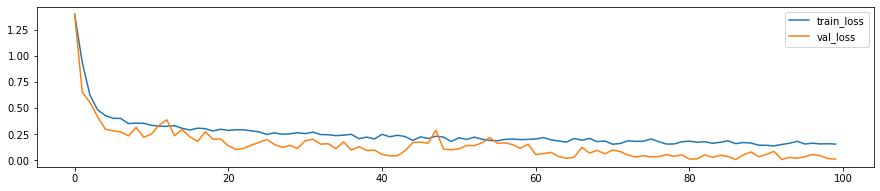
\includegraphics[width=1\linewidth]{results/efficientnet-b5/training_loss_results.png}
		\caption{Đồ thị training loss, validation loss}
		\label{fig:writing-thesis}
	\end{figure}
	\begin{figure}[H]
		\centering
		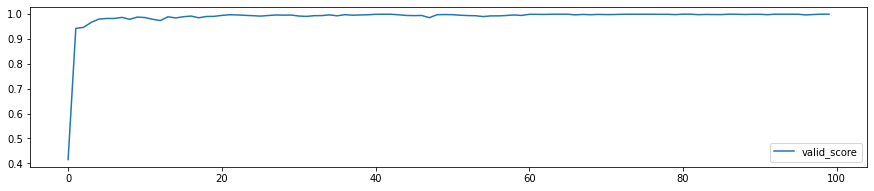
\includegraphics[width=1\linewidth]{results/efficientnet-b5/valid_score_results.png}
		\caption{Đồ thị Validation Score}
		\label{fig:writing-thesis}
	\end{figure}

	\textbf{Đường dẫn đến link Google Drive}:
	
	 \href{https://drive.google.com/drive/folders/1ObYuZYiq6aZ8Z1_HY08elUShmQ6LDb52?usp=sharing}{https://drive.google.com/drive/folders/1ObYuZYiq6aZ8Z1\_HY08elUShmQ6LDb52?usp=sharing}
	 
	 
	\textbf{Đường dẫn đến link Github}:
	
	\href{https://github.com/nhutnamhcmus/ml-lab-02-classification}{https://github.com/nhutnamhcmus/ml-lab-02-classification}
	
	
	\section{Phụ lục}
	
	\subsection{A. Transfer Learning - Phương pháp Học chuyển giao}
	Mô hình được đào tạo trước là một mạng đã lưu đã được đào tạo trước đó trên một tập dữ liệu lớn, thường là trong một nhiệm vụ phân loại hình ảnh quy mô lớn. Bạn có thể sử dụng mô hình được đào tạo trước như hiện tại hoặc sử dụng học chuyển giao để tùy chỉnh mô hình này cho một nhiệm vụ nhất định.
	
	Học chuyển giao (Transfer Learning) là một phương pháp Học Máy áp dụng kiến thức đã học được từ vấn đề này trong miền nguồn $ D_{S} $ với tác vụ nguồn $ T_{S}$ chuyển sang vấn đề khác - miền đích $ D_{T} $. Đề xuất của Chuyển giao Học tập là cải thiện chức năng học tập $f_{T}(.)$ Trong nhiệm vụ mục tiêu $ T_{T} $ trên miền mục tiêu $D_{T}$
	
	Đây là một cách tiếp cận phổ biến trong học sâu, trong đó các mô hình được đào tạo trước được sử dụng làm điểm khởi đầu cho các nhiệm vụ xử lý ngôn ngữ tự nhiên và thị giác máy tính với nguồn lực máy tính và thời gian khổng lồ cần thiết để phát triển các mô hình mạng nơ-ron cho những vấn đề này và từ những bước tiến lớn trong kỹ năng mà họ cung cấp về các vấn đề liên quan.
	
	\begin{figure}[H]
		\centering
		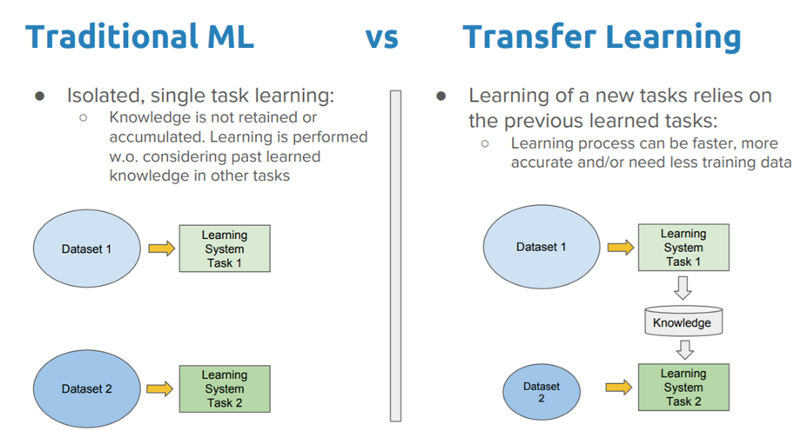
\includegraphics[width=1\linewidth]{architecture/traditional_ml_transfer_learning.png}
		\caption{A Comparision Traditional Machine Learning and Transfer Learning}
		\label{fig:writing-thesis}
	\end{figure}
	Có hai cách tiếp cận phổ biến cho phép chúng ta sử dụng học chuyển giao (Transfer Learning) cho các vấn đề mô hình dự đoán của riêng chúng ta.
	\begin{itemize}
		\item Develop Model Approach
		\item Pre-trained Model Approach
	\end{itemize}
	Với hướng tiếp cận Pre-trained Model Approach, ta có 3 cách tiếp cận khác nhau
	\begin{itemize}
		\item Select Source Model: Một mô hình nguồn được huấn luyện trước được chọn từ các mô hình có sẵn. Nhiều tổ chức nghiên cứu phát hành các mô hình trên các bộ dữ liệu lớn và đầy thách thức có thể được đưa vào nhóm các mô hình ứng viên để từ đó lựa chọn.
		\item Reuse Model: Mô hình được huấn luyện  trước của mô hình sau đó có thể được sử dụng làm điểm khởi đầu cho một mô hình về nhiệm vụ quan tâm thứ hai. Điều này có thể liên quan đến việc sử dụng tất cả hoặc các phần của mô hình, tùy thuộc vào kỹ thuật mô hình hóa được sử dụng.
		\item Tune Model: Theo tùy chọn, mô hình có thể cần được điều chỉnh hoặc tinh chỉnh dựa trên dữ liệu cặp đầu vào - đầu ra có sẵn cho nhiệm vụ quan tâm.
	\end{itemize}
	
	Loại thứ hai là Học tập chuyển giao phương pháp tiếp cận theo mô hình được đào tạo trước phổ biến trong lĩnh vực Học sâu.
	
	Trong phân trình bày bài báo, chúng em sử dụng một cách tiếp cận sử dụng Học chuyển giao (Transfer Learning) như một bước khởi đầu cơ bản, bằng cách sử dụng ResNet50
	\begin{figure}[H]
		\centering
		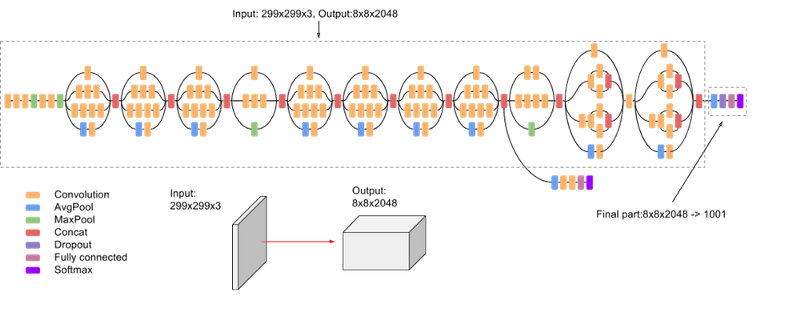
\includegraphics[width=1\linewidth]{architecture/Transfer_learning_as_a_starting_point.png}
		\caption{A Comparision Traditional Machine Learning and Transfer Learning}
		\label{fig:writing-thesis}
	\end{figure}
	Phương pháp học chuyển giao (Transfer Learning) là một tối ưu hóa, một con đường tắt để tiết kiệm thời gian hoặc đạt được hiệu suất tốt hơn.
	
	Nói chung, không có gì rõ ràng là sẽ có lợi khi sử dụng học chuyển giao trong miền cho đến khi mô hình đã được phát triển và đánh giá. Nhưng nó mang lại cho chúng ta một số lợi ích
	\begin{itemize}
		\item Higher start - Điểm bắt đầu tốt hơn
		\item Higher slope - Những hệ số tốt hơn
		\item Higher asymptote
	\end{itemize}
	\begin{figure}[H]
		\centering
		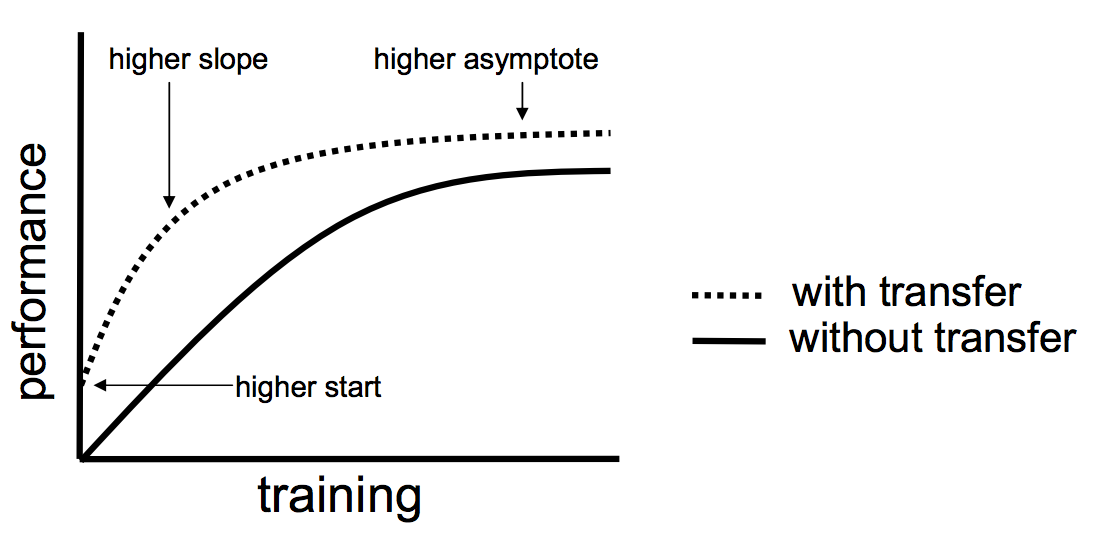
\includegraphics[width=1\linewidth]{architecture/performance_transfer_learning.png}
		\caption{A Comparision Traditional Machine Learning and Transfer Learning}
		\label{fig:writing-thesis}
	\end{figure}
	\subsection{B. Residual Networks - Mạng phần dư}
	ResNet là từ viết tắt của Residual Network được giới thiệu vào năm 2015 bởi Kaiming He, Xiangyu Zhang, Shaoqing Ren và Jian Sun trong bài báo của họ "Deep Residual Learning for Image Recognition". Mô hình ResNet cực kỳ thành công đã giành được vị trí đầu tiên trong cuộc thi phân loại ILSVRC 2015 với tỷ lệ lỗi top 5 là 3,57 \% (Mô hình tổng hợp). Không chỉ ILSVRC 2015 mà nó còn giành chiến thắng trong cuộc thi COCO 2015 về ImageNet Detection, ImageNet localization, Coco detection và Coco segmentation. Resercher thay thế các lớp VGG-16 trong Faster R-CNN bằng ResNet-101 và họ đã quan sát thấy sự cải thiện tương đối là 28 \%. Hiện tại, Mô hình ResNet có nhiều phiên bản như ResNet-18, ResNet-34, ResNet-50, ResNet-101, ResNet-152 ...
	
	Một vấn đề xảy ra khi xây dựng mạng CNN với hàng nghìn lớp phức tạp là Vấn đề Vanishing Gradient - Biến mất dốc đạo hàm, dẫn đến quá trình học, huấn luyện không tốt. Để cải thiện độ chính xác và hiệu suất, chúng tôi xếp chồng một số lớp bổ sung trong mạng Học Sâu với hy vọng rằng việc thêm nhiều lớp hơn để các lớp này dần dần học được các tính năng phức tạp hơn. Nhưng người ta thấy rằng có một ngưỡng tối đa về độ sâu với mô hình mạng neural truyền thống.
	\begin{figure}[H]
		\centering
		\includegraphics[width=1\linewidth]{architecture/Vanishing_Gradient.png}
		\caption{RVanishing Gradient Problem - Deep Residual Learning for Image Recognition}
		\label{fig:writing-thesis}
	\end{figure}
	Vấn đề đào tạo các mạng rất sâu này đã được giảm bớt với sự ra đời của ResNet hoặc các mạng còn lại và các mô hình Resnets này được tạo thành từ các Khối Residual Blocks.
	\begin{figure}[H]
		\centering
		\includegraphics[width=1\linewidth]{architecture/residual_learning_building_block.png}
		\caption{Residual Blocks - Deep Residual Learning for Image Recognition}
		\label{fig:writing-thesis}
	\end{figure}
	\begin{figure}[H]
		\centering
		\includegraphics[width=0.75\linewidth]{architecture/resnetwork.jpg}
		\caption{Residual Learning - Deep Residual Learning for Image Recognition}
		\label{fig:writing-thesis}
	\end{figure}
	Trong ResNets, có một kết nối trực tiếp từ một lớp này sang lớp khác mà bỏ qua một số lớp (có thể khác nhau ở các kiểu máy khác nhau) ở giữa. Chúng tôi gọi nó là 'skip connection' và nó là cốt lõi của Khối Residual Blocks. Đối tượng của kết nối bỏ qua, đầu ra của lớp không giống nhau. Nếu không bỏ qua kết nối, giá trị đầu vào $\textbf {x}$ sẽ được nhân với trọng số của lớp, sau đó thêm độ lệch (thiên vị - bias).
	
	Dữ liệu đi qua hàm kích hoạt $\mathcal{F}(\textbf {x})$, từ đầu vào $\textbf{x}$ đến lớp trọng số 1 (weight layer 1), ReLu Layer, đến lớp trọng số 2 (weight layer 2) và chúng tôi nhận được kết quả đầu ra là $\mathcal{F}(\textbf{x}, {W_i})$. Với kết nối bỏ qua (skip connection), chúng ta nhận được công thức sau đây:
	$$\textbf{y} = \mathcal{F}(\textbf{x}, {W_i}) + W_{s}\textbf{x}$$
	\begin{figure}[H]
		\centering
		\includegraphics[width=0.65\linewidth]{architecture/resnet.png}
		\caption{Residual Learning - Deep Residual Learning for Image Recognition}
		\label{fig:writing-thesis}
	\end{figure}
	Một mô hình ResNet50 có thể được mô tả bằng các thông số dưới đây
	\begin{itemize}
		\item Zero-padding: Convolution (Conv1) với 64 filters với shape$(7,7)$, sử dụng stride$(2,2)$, BatchNorm, MaxPooling $(3,3)$
		\item Stage 1: Convolutional block dùng 3 filters với kích thước $64 \times 64 \times 256$, $f=3$, $s=1$. Ở đây có 2 Identity blocks với kích thước filter $64 \times 64 \times 256$, $f=3$.
		\item Stage 2: Convolutional sử dụng 3 filters kích thước $128 \times 128 \times 512$, $f=3$,$s=2$. Ở đây có 3 Identity blocks với kích thước filter $128 \times 128 \times 512$, $f=3$.
		\item Stage 3: Convolutional sử dung 3 filter kích thước $256\times256\times1024$, $f=3$,$s=2$. Ở đây có 5 Identity blocks với kích thước filter $256\times256\times1024$, $f=3$.
		\item Stage 4: Convolutional uses 3 filter sizes $256\times256\times1024$, $f=3$,$s=2$. Ở đây có 5 Identity blocks với kích thước filter $256\times256\times1024$, $f=3$.
		\item Stage 5: Convolutional sử dụng 3 filters kích thước $512\times512\times2048$, $f=3$,$s=2$. Ở đây có 2 Identity blocks với kích thước filter $512\times512\times2048$, $f=3$.
		\item The 2D Average Pooling: với kích thước $(2, 2)$
		\item The Flatten: flatt data
		\item Fully Connected (Dense): sử dụng Softmax activation function.
	\end{itemize}
	\begin{figure}[H]
		\centering
		\includegraphics[width=0.85\linewidth]{architecture/The-architecture-of-ResNet50-and-deep-learning-model-flowchart-a-b-Architecture-of.png}
		\caption{The Architecture of ResNet50 - Deep Learning Model flowchart}
		\label{fig:writing-thesis}
	\end{figure}
	\subsection{C. EfficientNet}
	\textbf{Giới thiệu chung về EfficientNet}
	
	Convolutional neural networks (CNNs) thường được phát triển với chi phí tài nguyên cố định và sau đó được mở rộng để đạt được độ chính xác tốt hơn khi có nhiều tài nguyên hơn. Ví dụ: ResNet có thể được mở rộng từ ResNet-18 đến ResNet-200 bằng cách tăng số lớp và gần đây, GPipe đã đạt được độ chính xác top 1 của ImageNet là 84,3\% bằng cách tăng tỷ lệ CNN cơ sở lên hệ số bốn. Mặc dù các phương pháp này cải thiện độ chính xác, nhưng chúng thường yêu cầu điều chỉnh thủ công và chưa có một phương pháp cụ thể
	
	Trong bài báo ICML 2019 "EfficientNet: Rethinking Model Scaling for Convolutional Neural Networks" nhóm tác giả Mingxing Tan, Quoc V. Le đề xuất một phương pháp mở rộng mô hình mới sử dụng hệ số kép đơn giản nhưng hiệu quả cao để mở rộng quy mô CNN theo cách có cấu trúc hơn. Không giống như các phương pháp tiếp cận thông thường quy mô kích thước mạng một cách tùy ý, chẳng hạn như chiều rộng, chiều sâu và độ phân giải, phương pháp của chúng tôi chia tỷ lệ đồng nhất từng thứ nguyên với một tập hợp các hệ số tỷ lệ cố định. Được hỗ trợ bởi phương pháp chia tỷ lệ mới này và tiến bộ gần đây trên AutoML, chúng tôi đã phát triển một nhóm mô hình, được gọi là EfficientNets, vượt qua độ chính xác hiện đại với hiệu suất tốt hơn lên đến 10 lần (nhỏ hơn và nhanh hơn)
	
	\textbf{Thu phóng mô hình Convolutional Neural Networks}
	\begin{figure}[H]
		\centering
		\includegraphics[width=1\linewidth]{images/image4.png}
		\caption{The Architecture of EfficientNet}
		\label{fig:writing-thesis}
	\end{figure}
	\textbf{Thu phóng mô hình Convolutional Neural Networks theo chiều sâu - Depth Scaling}
	
	Thu phóng theo chiều sâu là một cách thông dụng nhất được sử dụng để thu phóng một mô hình CNN. Độ sâu có thể được thu phóng hay thu nhỏ bằng cách thêm hay bớt các lớp tương ứng. Ví dụ: ResNets có thể được mở rộng từ ResNet-50 đến ResNet-200 cũng như chúng có thể được thu nhỏ từ ResNet-50 thành ResNet-18.
	
	\textbf{Thu phóng mô hình Convolutional Neural Networks theo chiều rộng - Width Scaling}
	
	Thu phóng theo chiều rộng của mạng (theo như trong hình minh họa ta có thể hiểu là thêm dữ liệu đầu vào) cho phép các lớp học các đặc trưng chi tiết hơn.
	
	\textbf{Thu phóng mô hình Convolutional Neural Networks theo độ phân giải - Resolution Scaling}
	
	Tăng hoặc giảm độ phân giải của hình ảnh. Theo trực giác, khi tăng độ phân giải các đặc trưng dễ dàng được học hơn, kết quả sẽ tốt hơn nhưng thực ra, việc tính toán sẽ rất phức tạp, đôi khi lại không hiệu quả
	
	\textbf{Phương pháp}
	
	Theo nhóm tác giả quan sát các chiều của các mô hình thường không thu nhỏ/thu phóng đọc lập với nhau. Bởi vậy nên, theo trực giác của bản thân, nhóm tác giả cho rằng chúng ta cần phối hợp và cân bằng các kích thước tỷ lệ khác nhau — chiều rộng, chiều sâu và độ phân giải hình ảnh — hơn là chia tỷ lệ một chiều thông thường.
	
	Bước đầu tiên trong phương pháp chia tỷ lệ kết hợp là thực hiện tìm kiếm trên lưới để tìm mối quan hệ giữa các kích thước tỷ lệ khác nhau của mạng cơ sở dưới một hạn chế tài nguyên cố định (ví dụ: thêm 2x FLOPS). Điều này xác định hệ số tỷ lệ thích hợp cho từng thứ nguyên đã đề cập ở trên. Sau đó, nhóm tác áp dụng các hệ số đó để mở rộng mạng đường cơ sở đến kích thước mô hình mục tiêu mong muốn hoặc ngân sách tính toán.
	
	
	Phương pháp chia tỷ lệ kết hợp này luôn cải thiện độ chính xác và hiệu quả của mô hình để mở rộng các mô hình hiện có như MobileNet (+ 1,4\% độ chính xác của imagenet) và ResNet (+ 0,7\%), so với các phương pháp chia tỷ lệ thông thường.
	
	\textbf{Kiến trúc mạng EfficientNet}
	\begin{figure}[H]
		\centering
		\includegraphics[width=1\linewidth]{images/image2.png}
		\caption{The Architecture of EfficientNet }
		\label{fig:writing-thesis}
	\end{figure}
	
	\textbf{Hiệu năng của EfficientNet}
	
	\begin{figure}[H]
		\centering
		\includegraphics[width=0.5\linewidth]{images/image3.png}
		\caption{The Architecture of EfficientNet }
		\label{fig:writing-thesis}
	\end{figure}
	\nocite{*}
	\bibliography{references}\newpage\cleardoublepage
	\bibliographystyle{plain}
\end{document}